\documentclass[english,]{book}
\usepackage{lmodern}
\usepackage{amssymb,amsmath}
\usepackage{ifxetex,ifluatex}
\usepackage{fixltx2e} % provides \textsubscript
\ifnum 0\ifxetex 1\fi\ifluatex 1\fi=0 % if pdftex
  \usepackage[T1]{fontenc}
  \usepackage[utf8]{inputenc}
\else % if luatex or xelatex
  \ifxetex
    \usepackage{mathspec}
  \else
    \usepackage{fontspec}
  \fi
  \defaultfontfeatures{Ligatures=TeX,Scale=MatchLowercase}
\fi
% use upquote if available, for straight quotes in verbatim environments
\IfFileExists{upquote.sty}{\usepackage{upquote}}{}
% use microtype if available
\IfFileExists{microtype.sty}{%
\usepackage{microtype}
\UseMicrotypeSet[protrusion]{basicmath} % disable protrusion for tt fonts
}{}
\usepackage[margin=1in]{geometry}
\usepackage{hyperref}
\hypersetup{unicode=true,
            pdftitle={The Open Digital Archaeology Textbook Environment},
            pdfauthor={Shawn Graham, Neha Gupta, Michael Carter, \& Beth Compton},
            pdfborder={0 0 0},
            breaklinks=true}
\urlstyle{same}  % don't use monospace font for urls
\ifnum 0\ifxetex 1\fi\ifluatex 1\fi=0 % if pdftex
  \usepackage[shorthands=off,main=english]{babel}
\else
  \usepackage{polyglossia}
  \setmainlanguage[]{english}
\fi
\usepackage{longtable,booktabs}
\usepackage{graphicx,grffile}
\makeatletter
\def\maxwidth{\ifdim\Gin@nat@width>\linewidth\linewidth\else\Gin@nat@width\fi}
\def\maxheight{\ifdim\Gin@nat@height>\textheight\textheight\else\Gin@nat@height\fi}
\makeatother
% Scale images if necessary, so that they will not overflow the page
% margins by default, and it is still possible to overwrite the defaults
% using explicit options in \includegraphics[width, height, ...]{}
\setkeys{Gin}{width=\maxwidth,height=\maxheight,keepaspectratio}
\IfFileExists{parskip.sty}{%
\usepackage{parskip}
}{% else
\setlength{\parindent}{0pt}
\setlength{\parskip}{6pt plus 2pt minus 1pt}
}
\setlength{\emergencystretch}{3em}  % prevent overfull lines
\providecommand{\tightlist}{%
  \setlength{\itemsep}{0pt}\setlength{\parskip}{0pt}}
\setcounter{secnumdepth}{5}
% Redefines (sub)paragraphs to behave more like sections
\ifx\paragraph\undefined\else
\let\oldparagraph\paragraph
\renewcommand{\paragraph}[1]{\oldparagraph{#1}\mbox{}}
\fi
\ifx\subparagraph\undefined\else
\let\oldsubparagraph\subparagraph
\renewcommand{\subparagraph}[1]{\oldsubparagraph{#1}\mbox{}}
\fi

%%% Use protect on footnotes to avoid problems with footnotes in titles
\let\rmarkdownfootnote\footnote%
\def\footnote{\protect\rmarkdownfootnote}

%%% Change title format to be more compact
\usepackage{titling}

% Create subtitle command for use in maketitle
\newcommand{\subtitle}[1]{
  \posttitle{
    \begin{center}\large#1\end{center}
    }
}

\setlength{\droptitle}{-2em}
  \title{The Open Digital Archaeology Textbook Environment}
  \pretitle{\vspace{\droptitle}\centering\huge}
  \posttitle{\par}
  \author{Shawn Graham, Neha Gupta, Michael Carter, \& Beth Compton}
  \preauthor{\centering\large\emph}
  \postauthor{\par}
  \predate{\centering\large\emph}
  \postdate{\par}
  \date{2017-03-14}


\begin{document}
\maketitle

{
\setcounter{tocdepth}{1}
\tableofcontents
}
\chapter*{notice}\label{notice}
\addcontentsline{toc}{chapter}{notice}

This volume goes hand-in-glove with a computational environnent built on
the DHBox.

THIS IS A DRAFT VERSION; it's not even version 0.1 yet. It is filled
with errors, omissions, and non-sequiturs.

\begin{figure}[htbp]
\centering
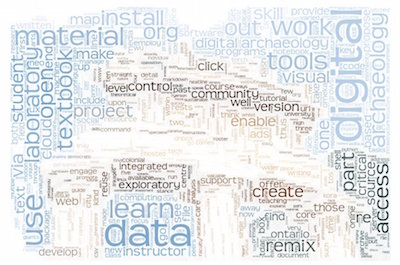
\includegraphics{images/word-cloud-proposal.jpg}
\caption{A word cloud image of the original ODATE proposal, arranged to
mimic a photograph of the temple of Athena Pronaos at Delphi}
\end{figure}


\includegraphics{images/by-nc-sa.png}\\
The online version of this book is licensed under the
\href{http://creativecommons.org/licenses/by-nc-sa/4.0/}{Creative
Commons Attribution-NonCommercial-ShareAlike 4.0 International License}.

\chapter*{About the Authors}\label{about-the-authors}
\addcontentsline{toc}{chapter}{About the Authors}

\subsection*{Shawn Graham}\label{shawn-graham}
\addcontentsline{toc}{subsection}{Shawn Graham}

Shawn Graham trained in Roman archaeology but has become over the years
a digital archaeologist and digital humanist. He is currently an
associate professor in the \href{http://carleton.ca}{Department of
History at Carleton University in Ottawa Canada}. He keeps an open lab
notebook of his research and experiments in digital history and
archaeology at his research blog,
\href{http://electricarchaeology.ca}{electricarchaeology}. He can be
found on Twitter at
\href{http://twitter.com/electricarchaeo}{electricarchaeo}. His teaching
explores methods and digital approaches at all levels, including
seminars in the collaborative MA Digital Humanities program as well as
in the MA Public History program. His research interests include
augmented reality and virtual reality in the service of landscape
archaeology, video games about the past, and agent based modeling.

\subsection*{Neha Gupta}\label{neha-gupta}
\addcontentsline{toc}{subsection}{Neha Gupta}

blah

\subsection*{Michael Carter}\label{michael-carter}
\addcontentsline{toc}{subsection}{Michael Carter}

blah

\subsection*{Beth Compton}\label{beth-compton}
\addcontentsline{toc}{subsection}{Beth Compton}

blah

\subsection*{Editorial Board}\label{editorial-board}
\addcontentsline{toc}{subsection}{Editorial Board}

Katharine Cook, University of Victoria

Ethan Watrall, Michigan State University

Daniel Pett, The British Museum

Eric Kansa, Open Context \& The Alexandria Archive Institute

Kathleen Fitzpatrick, Modern Language Association

\chapter*{Getting Started}\label{getting-started}
\addcontentsline{toc}{chapter}{Getting Started}

We wrote this text with a particular kind of student in mind. We
imagined this student as having already taken a first year introductory
course to archaeology, of the kind that surveys the field, its history,
and its principle methods and theoretical positions. Very few courses of
that kind include any depth in digital methods and theory, which is
understandable when we look at the incredible variety of archaeological
work, skills, and interests! Digital work is every bit as diverse as
other kinds of archaeology, but it also presents its own particular
challenges. One of these is the anxiety that comes when one first
approaches the computer for anything more complex than word processing
or a bit of social media. `What happens if I break it?'; `I'm not
techy!'; `If I wanted to do computers, I wouldn't have gone into this!'
are all actual student concerns that we have heard in our various
classrooms.

It'll be ok.

We take a pedagogical perspective that focuses on the learning that
happens when we make things, when we experiment or otherwise play around
with materials and computing, and especially, when/if things break. It's
a perspective that finds value in `failing gloriously', in trying to
push ourselves beyond our comfort level. The only thing that you will
need therefore to be successful in learning some of the basic issues
around digital archaeology is a willingness to consider why things
didn't work the way they ought to have, and a web browser. We built this
textbook with its very own digital archaeology computer built right in!
There's nothing you can break on your own machine, nor does your machine
have to be very powerful. If you want, you can even download and install
ODATE on a desktop computer to use as your very own digital archaeology
laboratory.

\section*{How to use this text}\label{how-to-use-this-text}
\addcontentsline{toc}{section}{How to use this text}

Each section in this book is broken down into an overview or discussion
of the main concepts, and then followed up with skill-building
exercises. The computational environment, when you log into it, is set
to expire after three hours - so you really ought to work through the
sections on \protect\hyperlink{github-version-control}{Github \& Version
Control} and
\protect\hyperlink{open-notebook-research-scholarly-communication}{Open
Notebook Research \& Scholarly Communication} so you'll be able to get
your work and data out of ODATE and onto space that you control. The
best way to use this book is to make sure you have at least one hour
blocked out to read through a section, and then two hours to go through
the section again if you're working on the exercises.

Do you notice that stripe down the side of the screen at the right?
That's a tool-bar for annotating the text, using a tool called
\texttt{Hypothes.is}. If you highlight any text (go ahead, highlight
that phrase right now by right-clicking and dragging your mouse!) a
little pop-up will ask you if you want to annotate or highlight the
text. If you choose annotate, a writing pane will open on the right.
Using the Hypothesis tool requires a reader to create a login and
account with Hypothesis, which is managed by the Hypothesis site, not
us.

By default, such annotations are made public. Private annotations can
only be viewed by the particular individual who made them. All
annotations (both public and private) have their own unique URL and can
be collated in various ways using the Hypothesis API (here's an
\href{http://jonudell.net/h/facet.html}{example}). Please tag your
annotation with \texttt{odate} to allow easy curating of the public
annotations.

Please note that any public annotations can be read by any other reader.
These can also be responded to, as well - which might make a great
classroom activity! A class can create group annotations which are only
visible to participants in that group
(\href{https://hypothes.is/blog/introducing-groups/}{instructions
here}). Annotation is a tool for research; personal reaction to anything
we've written in ODATE should be done via the reader's blog while
leaving an annotation on ODATE linking to the blog piece. Because the
API or `application programming interface' for Hypothesis allows one to
retrieve annotations programmatically, there is a growing world of
scripts and plugins for managing or retrieving those annotations. Kris
Shaffer has created a Wordpress plugin to pull annotations to a new
Wordpress post
(\href{http://pushpullfork.com/2016/08/hypothesis-aggregator/}{details
are linked here}), which might be another great option for a class blog
working through ODATE.

Over time, the parts of the text that are heavily annotated will look as
if someone has gone over them with a yellow highlighter. You can use
this to help guide your reading - perhaps that's a part where many
people had problems, or perhaps it's a part that sparked a really
interesting discussion! Group annotation like this promotes `active
reading', which means that you're more likely to retain the discussion.

Finally, if you'd rather not read this as a web page, you can grab a pdf
copy by pressing the download button above (the downwards-facing arrow
icon) and printing out just the bits you want or need. If you'd rather
read this text via an e-reader or iBooks or similar, the download link
will also give you an ePub version. Individuals who use a screenreader
or other assistive device might prefer to work with the pdf or epub
versions. Please do let us know if there is any way we can make this
text more accessible for users with particular needs. Since this text is
fundamentally a series of plain-text files that we then manipulate to
create these different outputs, it should be straightforward for us to
adapt accordingly!

\section*{How to contribute changes, or make your own
version}\label{how-to-contribute-changes-or-make-your-own-version}
\addcontentsline{toc}{section}{How to contribute changes, or make your
own version}

Perhaps your professor has assigned a portion of this text to your
class, with the instruction to improve it. Do you see the edit button at
the top of the screen (it looks like a little square with a pencil)? If
you click on that, and you have an account on Github (and you're signed
in), you will grab a copy of this entire text (but not the computational
part; the source code for that is \href{insert-the-link}{here instead})
that you can then edit. If you want, you can also make a
\texttt{pull-request} to us, asking us to fold your changes into our
textbook. We welcome these suggestions! Since this book has a
creative-commons license, you are welcome to expand and build upon this
as you wish, but do cite and link back to the original version.

\section*{How to access and use the computational
environment}\label{how-to-access-and-use-the-computational-environment}
\addcontentsline{toc}{section}{How to access and use the computational
environment}

link to site, instructions, also repo, also dhbox-on-a-stick

\section*{Colophon}\label{colophon}
\addcontentsline{toc}{section}{Colophon}

This text was created using the \href{http://bookdown.org}{Bookdown}
package for R Markdown. \href{http://rmarkdown.rstudio.com/}{R Markdown}
is a variant of the simple
\href{https://daringfireball.net/projects/markdown/}{Markdown format}
created by John Gruber. That is to say, at its core this text is a
series of simple text-files marked up with simple markers of syntax like
\texttt{\#} marks to indicate headings and so on. R Markdown allows us
to embed code snippets within the text that an interpreter, like
\href{https://www.rstudio.com/}{R Studio}, knows how to run, such that
the results of the calculations become embedded in the surrounding
discussion! This is a key part of making research more open and more
reproducible, and which you'll learn more about in chapter one.

The sequence of steps to produce a Bookdown-powered site looks like
this:

\begin{enumerate}
\def\labelenumi{\arabic{enumi}.}
\tightlist
\item
  create a new project in RStudio (we typically create a new project in
  a brand new folder)
\item
  run the following script to install Bookdown:
\end{enumerate}

\begin{verbatim}
install.packages("devtools")
devtools::install_github("rstudio/bookdown")
\end{verbatim}

\begin{enumerate}
\def\labelenumi{\arabic{enumi}.}
\setcounter{enumi}{2}
\tightlist
\item
  create a new textfile with \texttt{metadata} that describe how the
  book will be built. The metadata is in a format called \texttt{YAML}
  (`yet another markup language') that uses keys and values that get
  passed into other parts of Bookdown:
\end{enumerate}

\begin{verbatim}
title: "The archaeology of spoons"
author: "Graham, Gupta, Carter, & Compton"
date: "July 1 2017"
description: "A book about cocleararchaeology."
github-repo: "my-github-account/my-project"
cover-image: "images/cover.png"
url: 'https\://my-domain-ex/my-project/'
bibliography: myproject.bib
biblio-style: apa-like
link-citations: yes
\end{verbatim}

This is the only thing you need to have in this file, which is saved in
the project folder as \texttt{index.Rmd}.

\begin{enumerate}
\def\labelenumi{\arabic{enumi}.}
\setcounter{enumi}{3}
\item
  Write! We write the content of this book as text files, saving the
  parts in order. Each file should be numbered
  \texttt{01-introduction.Rmd}, \texttt{02-a-history-of-spoons.Rmd},
  \texttt{03-the-spoons-of-site-x.Rmd} and so on.
\item
  Build the book. With Bookdown installed, there will be a `Build Book'
  button in the R Studio build pane. This will generate the static html
  files for the book, the pdf, and the epub. All of these will be found
  in a new folder in your project, \texttt{\_book}. There are many more
  customizations that can be done, but that is sufficient to get one
  started.
\end{enumerate}

\subsection*{The computational
environment}\label{the-computational-environment}
\addcontentsline{toc}{subsection}{The computational environment}

The computational environment we are using is a fork of the
\href{http://dhbox.org}{DhBox} project from CUNY, led by Stephen
Zweibel, Patrick Smyth Developer, Jojo Karlin, and Matthew K. Gold.
DHBox requires Ubuntu \textgreater{}= 14.04 and Python 2.7x. We run it
at Carleton courtesy of the School of Computer Science, Andrew Pullin,
Peter Choynowski, and Doug Howe, via
\href{https://www.openstack.org/}{OpenStack} and
\href{https://www.docker.com/}{Docker}. A version of DHBox that can be
run from a USB stick can be found
\href{https://github.com/DH-Box/dh-usb}{here} and is worth exploring!

\chapter*{Welcome!}\label{welcome}
\addcontentsline{toc}{chapter}{Welcome!}

Digital archaeology as a field rests upon the creative use of primarily
open-source and/or open-access materials to archive, reuse, visualize,
analyze and communicate archaeological data. This reliance on
open-source and open-access is a political stance that emerges in
opposition to archaeology's past complicity in colonial enterprises and
scholarship; digital archaeology resists the digital neo-colonialism of
Google, Facebook, and similar tech giants that typically promote
disciplinary silos and closed data repositories. Specifically, digital
archaeology encourages innovative, reflective, and critical use of open
access data and the development of digital tools that facilitate
linkages and analysis across varied digital sources.

To that end, this document you are reading is integrated with a
cloud-based digital exploratory laboratory of multiple cloud-computing
tools with teaching materials that instructors will be able to use
`out-of-the-box' with a single click, or to remix as circumstances
dictate. Part of our inspiration comes from the `DHBox' project from
CUNY (City University of New York, \href{http://dhbox.org}{(link)}, a
project that is creating a `digital humanities laboratory' in the cloud.
While the tools of the digital humanities are congruent with those of
digital archaeology, they are typically configured to work with texts
rather than material culture in which archaeologists specialise. The
second inspiration is the open-access guide `The Programming Historian',
which is a series of how-tos and tutorials
\href{http://programminghistorian.org}{(link)} pitched at historians
confronting digital sources for the first time. A key challenge scholars
face in carrying out novel digital analysis is how to install or
configure software; each `Programming Historian' tutorial therefore
explains in length and in detail how to configure software. The present
e-textbook merges the best of both approaches to create a singular
experience for instructors and students: a one-click digital laboratory
approach, where installation of materials is not an issue, and with
carefully designed tutorials and lessons on theory and practice in
digital archaeology.

This is not a textbook about learning how to code. Rather, it is about
instilling the habits of thought that will enable success when
confronted with digital novelty, the habits of thought that will enable
you to determine how to work with digital materials, and the habits of
thought that permit you to see where and when digital approaches will
make the difference in your research. Skills change; techniques evolve;
new tools emerge. Habits of thought are hard to cultivate but have
staying power!

\chapter{Going Digital}\label{going-digital}

\begin{quote}
Digital archaeology should exist to assist us in the performance of
archaeology as a whole. It should not be a secret knowledge, nor a
distinct school of thought, but rather simply seen as archaeology done
well, using all of the tools available to and in better recovering,
understanding and presenting the past. In the end, there is no such
thing as digital archaeology. What exists, or at least what should
exist, are intelligent and practical ways of applying the use of
computers to archaeology that better enable us to pursue both our
theoretical questions and our methodological applications. (Evans, Daly,
and MyiLibrary \protect\hyperlink{ref-evans_digital_2006}{2006})
\end{quote}

While we agree with the first part of the sentiment, the second part is
rather up for debate. We believe that there \emph{is} such a thing as
digital archaeology. Digital tools exist in a meshwork of legal and
cultural obligations, and moreso than any other tool humans have yet
come up with, have the capability to exert their own agency upon the
user. Digital tools and their use are not theory-free nor without
theoretical implications. There is no such thing as neutral, when
digital tools are employed. This is why digital archaeology is - or
should be - a distinct subfield of the wider archaeological project.

In a conversation initiated on Twitter on March 10, 2017, Graham asked
the question, `is digital archaeology the same as using computers in
archaeology?' REF.
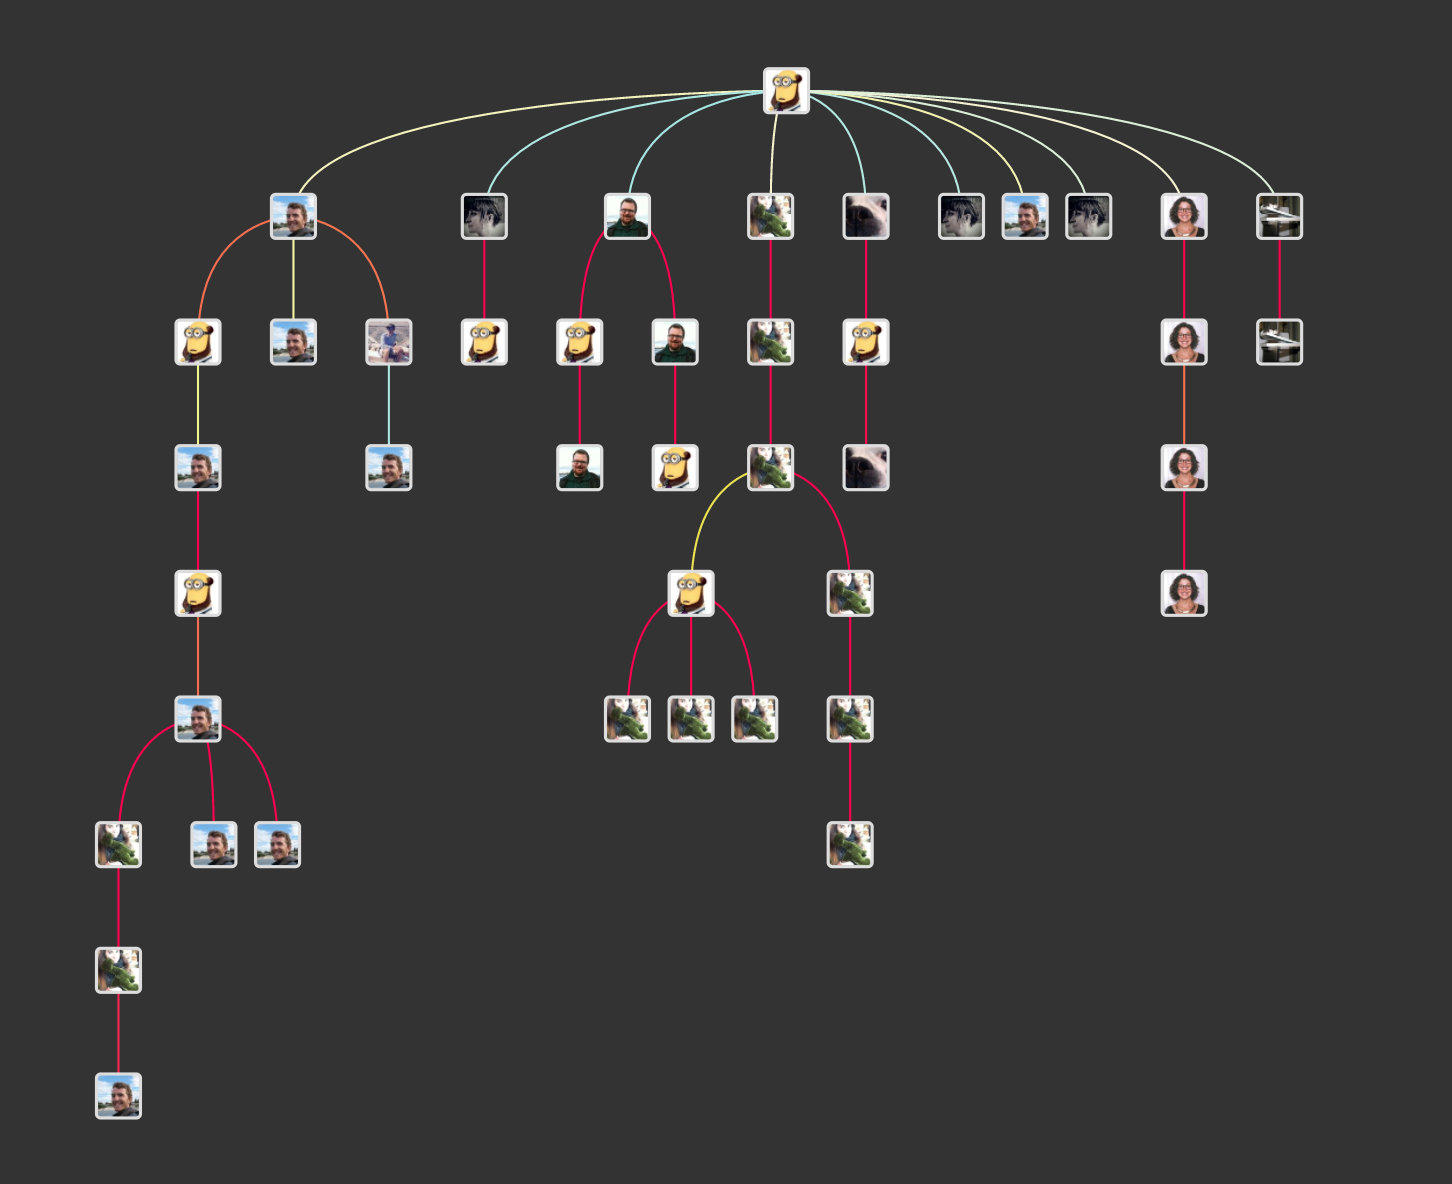
\includegraphics{Treeverse-representation-of-what-is-digital-archaeology-conversation-2017-03-10-at-11.56.07-AM}
The resulting conversation ranged widely over everything from the topic
of study (ref tinysapiens ref) to the ways in which computational power
enables the researcher to ask questions that were not previously
feasible to ask (ref CD Wren). Other researchers sounded a note of
caution against the kind of `technological fetishism' (ref Lorna) that
digital work can often fall pray to, especially given the larger issues
of gender and `solutionitis' that emerge given the white, 20-35 year old
demographic of many tech workers (for criticisms of technological
solutionism or utopianism in archaeology, see the work of Colleen Morgan
(ref phd thesis) Joyce, Tringham, Morozov, Kansa ). Others sounded a
warning that to think of digital archaeology as something distinct from
archaeology risks `going the way of DH' and instead appealed for a
holistic understanding (ref Gruber). Dimitri Naskiss \ldots{}blah, we're
all digital\ldots{}

Hanna Marie Pageau succintly captured these issues, when over a series
of tweets (REF) she wrote,

\begin{quote}
`Digital archaeology has an obvious digital component. However, saying
it's simply using a computer is like saying being a computer scientist
means you use a computer to do science. There is an implied addition
{[}to the{]} topic of specific methods that brings you from an
archaeologist using a computer to being an archaeologist who studies
digital archaeology. I would argue that archaeogaming is the most
straight forward example. Because while gaming is usually thought of as
digital, it could study table top gaming and not technically be digital
in nature. However if you're studying ethics of representation in games
you're going from just using a computer as a tool to it being THE
medium.'
\end{quote}

In which case, an important aspect of digital archaeology that
differentiates it from the use of computing power to answer
archaeological questions is this question of purpose. In this section,
we take up this question beginning with the question of \emph{teaching}
digital approaches. We progress by suggesting that digital archaeology
is akin to work at the intersection of art and public archaeology and
digital humanities. We provide you the necessary basics for setting up
your own digital archaeological practice. Entrance into the world of
digital archaeology requires organizational ability and facility with
versioning files. It is allied with the practice of open notebook
science, and it attempts to future-proof by using the simplest file
formats and avoiding proprietary software where possible. These are the
basics on which the rest of digital archaeological practice is founded.

\section{So what is Digital
Archaeology?}\label{so-what-is-digital-archaeology}

If you are holding this book in your hands, via a device or on paper, or
looking at it on your desktop, you might wonder why we feel it necessary
to even ask the question. It is important at the outset to make the
argument that digital archaeology is not about `mere' tool use. Andrew
Goldstone in \emph{Debates in the Digital Humanities} discusses this
tension (Goldstone
\protect\hyperlink{ref-goldstone_teaching_2018}{2018}). He has found
(and Lincoln Mullen concurs with regard to his own teaching,(Mullen
\protect\hyperlink{ref-mullen_confirmation_2017}{2017})) that our
current optimism about teaching technical facility is misplaced. Tools
first, context second doesn't work. Alternatively, theory first doesn't
seem to work either. And finally, for anything to work at all, datasets
have to be curated and carefully pruned for their pedagogical value. We
can't simply turn students loose on a dataset (or worse, ask them to
build their own) and expect `learning' to happen.

Our approach in this volume is to resolve that seeming paradox by
providing not just the tools, and not just the data, but also the
computer itself. Archaeologically, this puts our volume in dialog with
the work of scholars such as Ben Marwick, who makes available with his
research the code, the dependencies, and sometimes, an entire virtual
machine, to enable other scholars to replicate, reuse, or dispute his
conclusions. We want you to reuse our code, to study it, and to improve
upon it. We want you to annotate our pages, and point out our errors.
For us, digital archaeology is not the mere use of computational tools
to answer archaeological questions. Rather, it is to enable the audience
for archaeological thinking to enter into conversation with us, and to
\emph{do} archaeology for themselves.

Digital archaeology is necessarily a public archaeology. This is its
principal difference with what has come before, for never forget, there
has been at least a half-century of innovative use of computational
power for archaeological knowledge building.

Ethan Watrall has drawn the histoy of computational archaeology/digital
archaeology all the way back to the pioneering work of James Deetz in
the 1960s, who used computers at MIT to perform stylistic analyses of
Arikara ceramics (Ethan Watrall
\protect\hyperlink{ref-watrall_archaeology_2017}{2017}, Deetz
(\protect\hyperlink{ref-deetz_dynamics_1965}{1965})). Most early
interest in computation for archaeology was centred on the potential for
computational databases, although ambition often out-stripped
capability. By the 1970s, serious efforts were being put into work to
build the infrastructural knowledge necessary to make and usefully query
archaeological datasets. One can see this concern play out by
considering a \texttt{topic\ model} (Shawn Graham
\protect\hyperlink{ref-shawn_graham_digital_2014}{2014}) of the early
volumes of the Computer Applications in Archaeology (a topic model is a
way of deducing latent patterns of discourse within text, based on
patternings of words (See Graham, Weingart, and Milligan
\protect\hyperlink{ref-graham_getting_2012}{2012})):

topic 1 -- computer, program, may, storage, then, excavation, recording,
all, into, form, using, retrieval, any, user, output, records, package,
entry, one, unit

topic 6: but, they, one, time, their, all, some, only, will, there,
would, what, very, our, other, any, most, them, even

topic 20: some, will, many, there, field, problems, may, but,
archaeologists, excavation, their, they, recording, however, record,
new, systems, most, should, need

The beginnings of the CAA are marked by hesitation and prognostication:
what \emph{are} computers for, in archaeology? There is a sense that for
archaeologists, computation is something that will be useful insofar as
it can be helpful for recording information in the field. By the 1980s
desktop computing was becoming sufficiently widespread that the use of
geographic information systems was feasible for more and more
archaeologists. The other `killer app' of the time was computer-aided
design, which allowed metric 3d reconstructions from the plans drawn on
site by excavators. Yet, computational resources were still limited
enough that computing was not something that one could merely `play'
with. Software was costly, computation took time, and training resources
were put into learning the proprietary packages that existed (rather
than coding knowledge). By the 1990s, the introduction of the cd-rom and
the shift in PC gaming technologies from primarily text-based to
graphical based games led to teaching simulations for archaeology, most
notably T. Douglas Price and Anne Birgitte Gebauer's \emph{Adventures in
Fugawiland}. Watrall identifies the emergence of the web as being not so
much a boon for computational archaeology as it was for public
archaeology (although the pioneering journal \emph{Internet Archaeology}
was first published in 1996); nevertheless, the birth of the web (which
it must be remembered is \emph{distinct from} and \emph{overlays} the
internet) allowed for a step-change in the effectiveness of the
dissemination of open-source software and code, including practices for
remote collaboration on code that are now beginning to percolate into
scholarly publication.

The 2000s have seen, insofar as digital archaeology is concerned, a
replay of the earlier episodes of computational archaeology,
concommitant with each subsequent web `revolution' (ie, so-called web
2.0, web 3.0 etc). Works such as (Evans, Daly, and MyiLibrary
\protect\hyperlink{ref-evans_digital_2006}{2006}) and (E. C. Kansa,
Kansa, and Watrall \protect\hyperlink{ref-kansa_archaeology_2011}{2011})
are broadly concerned more with questions of infrastructure and
training, while the more recent \emph{Mobilizing the Past} deal with
problems of training, and the ethical issues that the emerging digital
surveillance permitted by our networked society presents to the practice
of archaeology (and public archaeology). Perhaps the most promising new
digital technologies to emerge in recent years include methods for
linking open archaeological data via the web (ie, freeing various
`silos' of disciplinary knowledge so that the semantic connections
between them can be followed and queried) and various mixed-reality
approaches (virtual reality, augmented reality, 3d printing, and the
so-called internet of things or the practice of wiring everything that
can be wired to the web). The 2000s have also seen a growing realization
that our digital tools and their algorithmic biases not only permit
interesting questions to be asked about the past, but also inhibit
points of view or impose their own worldviews upon the past in ways that
may damage communities and/or scholarship. This reflective critique of
computation in the service of archaeology marks digital archaeology
within the ambit of the digital humanities (despite the division between
anthropological and humanistic archaeologies).

\subsection{Is digital archaeology part of the digital
humanities?}\label{is-digital-archaeology-part-of-the-digital-humanities}

In recent years - certainly the last decade - an idea called `the
digital humanities' has been percolating around the academy. It is a
successor idea to `humanities computing', but it captures that same
distinction between discussed above. Digital archaeology has developed
alongside the digital humanities, sometimes intersecting with it
(notably, there was a major archaeological session at the
annualinternational Alliance of Digital Humanities Organizations
(\href{http://adho.org/}{ADHO}) DH conference in 2013).

The various component organizations of the ADHO have been meeting in one
form or another since the 1970s; so too the Computer Applications in
Archaeology Conference has been publishing its proceedings since 1973.
Archaeologists have been running simulations, doing spatial analysis,
clustering, imaging, geophysicing, 3d modeling, neutron activation
analyzing, x-tent modeling , etc, for what seems like ages. Happily,
there is no one definition of `dh' that everyone agrees on (see the
various definitions collected at \url{http://definingdh.org/}; reload
the page to get a new definition). For us, a defining
\emph{characteristic} of DH work is that public use we discussed above.
But, another characteristic that we find useful to consider is the
\emph{purpose} to which computation is put in DH work. This means that
digital work also has to be situated in the contexts of power and access
and control (which sometimes means that digital work is
mis-characterised as being part of a `neo-liberal' agenda to reduce
knowledge work to base profit motifs, eg Brouiellet; more thoughtful
work about the confluence of the digital with neoliberalism may be found
in Caraher xxxx and Kansa xxxx and Greenspan xxx. We discuss the ethical
dimensions to digital work more fully in
\protect\hyperlink{the-ethics-of-big-data-in-archaeology}{The Ethics of
Big Data in Archaeology}.)

For us, a key difference between the kind of computational archaeology
of the last years of the twentieth century versus the emerging digital
archaeology of the last decade lie in the idea of the purpose behind the
computing power. Trevor Owens, a digital archivist, draws attention to
the purpose behind one's use of computational power -- generative
discovery versus justification of an hypothesis (tjowens
\protect\hyperlink{ref-tjowens_discovery_2012}{2012}). Discovery marks
out the digital humanist whilst justification signals the humanist who
uses computers. Discovery and justification are critically different
concepts. For Owens, if we are using computational power to deform our
texts, then we are trying to see things in a new light, to create new
juxtapositions, to spark new insight. Stephen Ramsay talks about this
too in Reading Machines (Ramsay
\protect\hyperlink{ref-ramsay_reading_2011}{2011}, 33), discussing the
work of Samuels and McGann, (Samuels and McGann
\protect\hyperlink{ref-samuels_deformance_1999}{1999}): ``Reading a poem
backward is like viewing the face of a watch sideways -- a way of
unleashing the potentialities that altered perspectives may reveal''.
This kind of reading of data (especially, but not necessarily, through
digital manipulation), does not happen very much at all in archaeology.
If `deformance' is a key sign of the digital humanities, then digital
archaeologists are not digital humanists. Owen's point isn't to signal
who's in or who's out, but rather to draw attention to the fact that:

\begin{quote}
When we separate out the the context of discovery and exploration from
the context of justification we end up clarifying the terms of our
conversation. There is a huge difference between ``here is an
interesting way of thinking about this'' and ``This evidence supports
this claim.''
\end{quote}

This is important in the wider conversation concerning how we evaluate
digital scholarship. We've used computers in archaeology for decades to
try to justify or otherwise connect our leaps of logic and faith,
spanning the gap between our data and the stories we'd like to tell. We
believe, on balance, that `digital archaeology' sits along this spectrum
between justification and discovery closer to the discovery end, that it
sits within the digital humanities and should worry less about
hypothesis testing, and concentrate more on discovery and generation, of
`interesting way{[}s{]} of thinking about this'.

Digital archaeology should be a prompt to make us `think different'.
Let's take a small example of how that might play out. It's also worth
suggesting that `play' as a strategy for doing digital work is a valid
methodology (see Ramsay
(\protect\hyperlink{ref-ramsay_reading_2011}{2011})). (And of course,
the ability to play with computing power is a function of Moore's law
governing the increase in computing power time: computing is no longer a
precious resource but something that can be `wasted'.)

\subsection{Archaeological Glitch Art}\label{archaeological-glitch-art}

Bill Caraher is a leading thinker on the implications and practice of
digital archaeology. In a post on archaeological glitch art (Caraher
\protect\hyperlink{ref-caraher_archaeological_2012}{2012}) Caraher
changed file extensions to fiddle about in the insides of images of
archaeological maps. He then looked at them again as images:

\begin{quote}
The idea \ldots{} is to combine computer code and human codes to
transform our computer mediated image of archaeological reality in
unpredictable ways. The process is remarkably similar to analyzing the
site via the GIS where we take the ``natural'' landscape and transform
it into a series of symbols, lines, and text. By manipulating the code
that produces these images in both random and patterned ways, we
manipulate the meaning of the image and the way in which these images
communicate information to the viewer. We problematize the process and
manifestation of mediating between the experienced landscape and its
representation as archaeological data.
\end{quote}

Similarly, Graham's work in representing archaeological data in sound (a
literal auditory metaphor) translates movement over space (or through
time) into a soundscape of tones (Graham
\protect\hyperlink{ref-graham_cacophony_2017}{2017}). This frees us from
the tyranny of the screen and visual modes of knowing that often occlude
more than they reveal (for instance, our Western-framed understanding of
the top of the page or screen as `north' means we privilege visual
patterns in the vertical dimension over the horizontal (Montello et al.
\protect\hyperlink{ref-montello_testing_2003}{2003})).

These playful approaches force us to rethink some of our norms of
communication, our norms of what archaeology can concern itself with. It
should be apparent that digital archaeology transcends mere `digital
skills' or `tool use'; but it also suffers from being `cool'.

\subsection{\texorpdfstring{The `cool'
factor}{The cool factor}}\label{the-cool-factor}

Alan Liu (Liu \protect\hyperlink{ref-liu_laws_2004}{2004}) wondered what
the role of the arts and humanities was in an age of knowledge work, of
deliverables, of an historical event horizon that only goes back the
last financial quarter. He examined the idea of `knowledge work' and
teased out how much of the driving force behind it is in pursuit of the
`cool'. Through a deft plumbing of the history of the early internet
(and in particular, riffing on Netscape's `what's cool?' page from 1996
and their inability to define it except to say that they'd know it when
they saw it), Liu argues that cool is `the aporia of information\ldots{}
cool is information designed to resist information\ldots{} information
fed back into its own signal to create a standing interference pattern,
a paradox pattern' (Liu \protect\hyperlink{ref-liu_laws_2004}{2004},
179). The latest web design, the latest app, the latest R package for
statistics, the latest acronym on Twitter where all the digital
humanists play: cool, and dividing the world.

That is, Liu argued that `cool' was amongst other things a politics of
knowledge work, a practice and ethos. He wondered how we might
`challenge knowledge work to open a space, as yet culturally sterile
(coopted, jejune, anarchistic, terroristic), for a more humane hack of
contemporary knowledge?' (Liu
\protect\hyperlink{ref-liu_laws_2004}{2004}, 9). Liu goes on to discuss
how the tensions of `cool' in knowledge work (for us, read: digital
archaeology) also intersects with an ethos of the unknown, that is, of
knowledge workers who work nowhere else somehow manage to stand outside
that system of knowledge production. (Is alt-ac `alt' partially because
it is the cool work?). This matters for us as archaeologists. There are
many `cool' things happening in digital archaeology that somehow do not
penetrate into the mainstream (such as it is). The utilitarian
dots-on-a-map were once cool, but are now pedestrian. The `cool' things
that could be, linger on the fringes. If they did not, they wouldn't be
cool, one supposes. They resist.

To get that more humane hack that Liu seeks, Liu suggests that the
historical depth that the humanities provides counters the shallowness
of cool:

\begin{quote}
The humanities thus have an explanation for the new arts of the
information age, whose inheritance of a frantic sequence of artistic
modernisms, postmodernisms, and post-postmodernists is otherwise only a
displaced encounter with the raw process of historicity. Inversely, the
arts offer the humanities serious ways of engaging -- both practically
and theoretically- with ``cool''. Together, the humanities and arts
might be able to offer a persuasive argument for the humane arts in the
age of knowledge work. (Liu \protect\hyperlink{ref-liu_laws_2004}{2004},
381).
\end{quote}

In which case, the emergence of digital archaeologists and historians in
the last decade might be the loci of the humane hacks -- if we move into
that space where we engage the arts. Indeed, the seminal anthropologist
Tim Ingold makes this very argument with reference to his own arc as a
scholar, `From Science to Art and Back Again':

\begin{quote}
Revisiting science and art: which is more ecological now? Why is art
leading the way in promoting radical ecological awareness? The goals of
today's science are modelling, prediction and control. Is that why we
turn to art to rediscover the humility that science has lost?
\end{quote}

We need to be making art. Digital archaeology naturally pushes in that
direction.

\subsection{Takeaways}\label{takeaways}

\begin{itemize}
\tightlist
\item
  Digital archaeology is a public archaeology
\item
  Digital archaeology is often about deformance rather than
  justification
\item
  In that deformative practice, it is in some ways extremely aligned
  with artistic ways of knowing
\item
  Digital archaeology is part of the digital humanities, and in many
  ways, presaged current debates and trends in that field.
\end{itemize}

All of these aspects of digital archaeology exist along a continuum. In
the remainder of this chapter, we give you a `boot-camp' to get you to
the point where you can begin to wonder about deformation and the public
entanglement with your work.

\subsection{Exercises}\label{exercises}

The first steps in going digital are quite easy. They are fundamentally
a question of maintaining some basic good habits. Everything else flows
from these three habits:

\begin{verbatim}
1. separate _what_ your write/create from _how_ you write it.
2. keep what you write/create under version control.
3. break tasks down into their smallest manageable bits
\end{verbatim}

Have you ever fought with Word or another wordprocessor, trying to get
things just right? Word processing is a mess. It conflates writing with
typesetting and layout. Sometimes, you just want to get the words out.
Othertimes, you want to make your writing as accessible as
possible\ldots{} but your intended recipient can't open your file,
because they don't use the same wordprocessor. Or perhaps you wrote up
some great notes that you'd love to have in a slideshow; but you can't,
because copying and pasting preserves a whole lot of extra gunk that
messes up your materials. Similarly, while many archaeologists will use
Microsoft Excel to manipulate tabular data (artifact measurements,
geochemistry data, and so on), Excel is well known for both
\href{https://github.com/jennybc/scary-excel-stories}{corrupting data}
and for being impossible to replicate (ie, the series of clicks to
manipulate or perform an analysis differ depending on the individual's
particular installation of Excel).

The answer is to separate your content from your tool, and your
analytical processes separate from your data. This can help keep your
thinking clear, but it also has a more nuts-and-bolts practical
dimension. \emph{A computer will always be able to read a text file}.
That is to say: you've futureproofed your material. Any researcher will
have old physical discs or disc drives or obsolete computers lying
around. It is not uncommon for a colleague to remark, `I wrote this in
Wordperfect and I can't open this any more'. Graham's MA thesis is
trapped on a 3.5" disc drive that was compressed using a now-obsolete
algorithm and it cannot be recovered. If, on the other hand, he had
written the text as a .txt file, and saved the data as .csv tables,
those materials would \emph{continue} to be accessible. If the way you
have manipulated or cleaned the data is written out as a
\texttt{script}, then a subsequent investigator (or even your future
self) can re-run the exact sequence of analysis, or re-write the script
into the equivalent steps in another analytical language.

A .txt file is simply a text file; a .csv is a text file that uses
commas to separate the text into columns. Similarly, a .md file is a
text file that uses things like \texttt{\#} to indicate headers, and
\texttt{\_} to show where italicized text starts and stops. A script, in
a play, tells you what to say and do. A \texttt{script} for a language
like \texttt{R} or \texttt{Python} does the same thing for the computer,
and has the advantage that it is human-readable and annotatable as well,
because its format \emph{is still a simple text file}. Scripts you might
encounter could have the \texttt{.r} or \texttt{.py} or \texttt{.sh}
file extensions. You can open these in a text editor and see what the
computer is being instructed to do. Annotations or comments in the
script can be set off in various ways, and help the researcher know what
is happening or is intended to happen at various points. Let's begin by
creating some simple text files to document our research process, in the
Markdown format.

\begin{enumerate}
\def\labelenumi{\arabic{enumi}.}
\tightlist
\item
  A nice place to practice writing in markdown that shows you
  immediately how your text might be rendered when turned into html,
  pdf, or Word doc is \href{http://dillinger.io}{Dillinger.io}. Go there
  now to try it out. Write a short piece on why you're interested in
  Digital Archaeology.
\end{enumerate}

\begin{enumerate}
\def\labelenumi{\alph{enumi}.}
\tightlist
\item
  Include a blockquote from the introduction to this book.
\item
  Include two links to an external site.
\item
  Embed an image.
\end{enumerate}

\begin{enumerate}
\def\labelenumi{\arabic{enumi}.}
\setcounter{enumi}{1}
\item
  In ODATE at the command line, you'll now write a markdown file using
  the built-in text editor \texttt{nano}. Everywhere in this book where
  you see the \texttt{\$} symbol, we mean for you to type whatever
  follows \emph{after} the \texttt{\$} at the command line. The
  \texttt{\$} is the \emph{prompt}. Enter the command
  \texttt{\$\ nano\ my-first-md-file.md}. This tells the machine to use
  the nano text editor to make a new file called
  \texttt{my-first-md-file.md} and to allow you to edit it right away.
  (If you just wanted to create an empty file, you could use
  \texttt{\$\ touch\ my-first-md-file.md}). The screen that opens is a
  simple text editor. Re-write what you wrote for \texttt{1} but add
  subheadings this time. To save your work, hit \texttt{ctrl+x}. Nano
  will ask you if you want to save changes; select \texttt{y}. It will
  then prompt you for a file name, but \texttt{my-first-md-file.md} will
  \emph{already} be inserted there, so just hit enter.
\item
  Make a new markdown file called `todo list' or similar. Use bullet
  points to break down what else you need to do this week. Each bullet
  point should have a sub-bullet with an actual \texttt{ACTION} listed,
  something that you can accomplish to get things done.
\end{enumerate}

** As you work through this book, we encourage you to write your
thoughts, observations, or results in simple text files.** This is good
practice whether or not you embark on a full-blown digital project,
because ultimately, if you use a computer in your research, you
\emph{have} gone digital.

\hypertarget{project-management-basics}{\section{Project Management
Basics}\label{project-management-basics}}

A digital project, whether in archaeology or in other fields, iterates
through the same basic steps. There is

\begin{verbatim}
1. finding data
2. fixing data
3. analyzing the data
4. communicating the story in the data
\end{verbatim}

Eighty percent of your time on any digital project will be invested in
cleaning up the data and documenting what you've done to it. But in
truth, a digital project begins long before we ever look at a data set
(or are given data to work with, if we're part of a larger project). How
do we formulate a research question or our exploration more generally?
How do we translate a gut feeling or intution or curiosity into
something that is \emph{operable}? REF Moretti on operationalizing
things

The four steps we identified above are cyclical; at any one time you
might be at a different stage of the process. Indeed, those four steps
could easily be subsumed under what Simon Appleford and Jennifer
Guiliano of \href{http://devdh.org}{devdh.org} identify as the `Best
Practice Principles Of Designing Your First Project.' For Appleford and
Guiliano, the outline of a project involves figuring out:

\begin{enumerate}
\def\labelenumi{\arabic{enumi}.}
\tightlist
\item
  the question, problem, or provocation
\item
  sources (primary, secondary)
\item
  analytical activity
\item
  audience
\item
  product
\end{enumerate}

Note that 4, audience, comes before 5, product. You must think of your
reader/user!

Let us imagine that we were inspired by Allison Mickel's piece, `Tracing
Teams, Texts, and Topics: Applying Social Network Analysis to Understand
Archaeological Knowledge Production at Çatalhöyük' (Mickel
\protect\hyperlink{ref-mickel_tracing_2016}{2016}).

We could frame a question: `What role do social networks play in the
development of knowledge production at my site?'

We could frame a problem: `Mickel's exploration of social networks
considered x, but not y.'

We could frame a provocation: `Social Network Analysis promises to
revolutionize our knowledge of the social contexts that underpin
archaeological fieldwork, putting this power in the hands of everyone
from the site director on down.'

\begin{figure}[htbp]
\centering
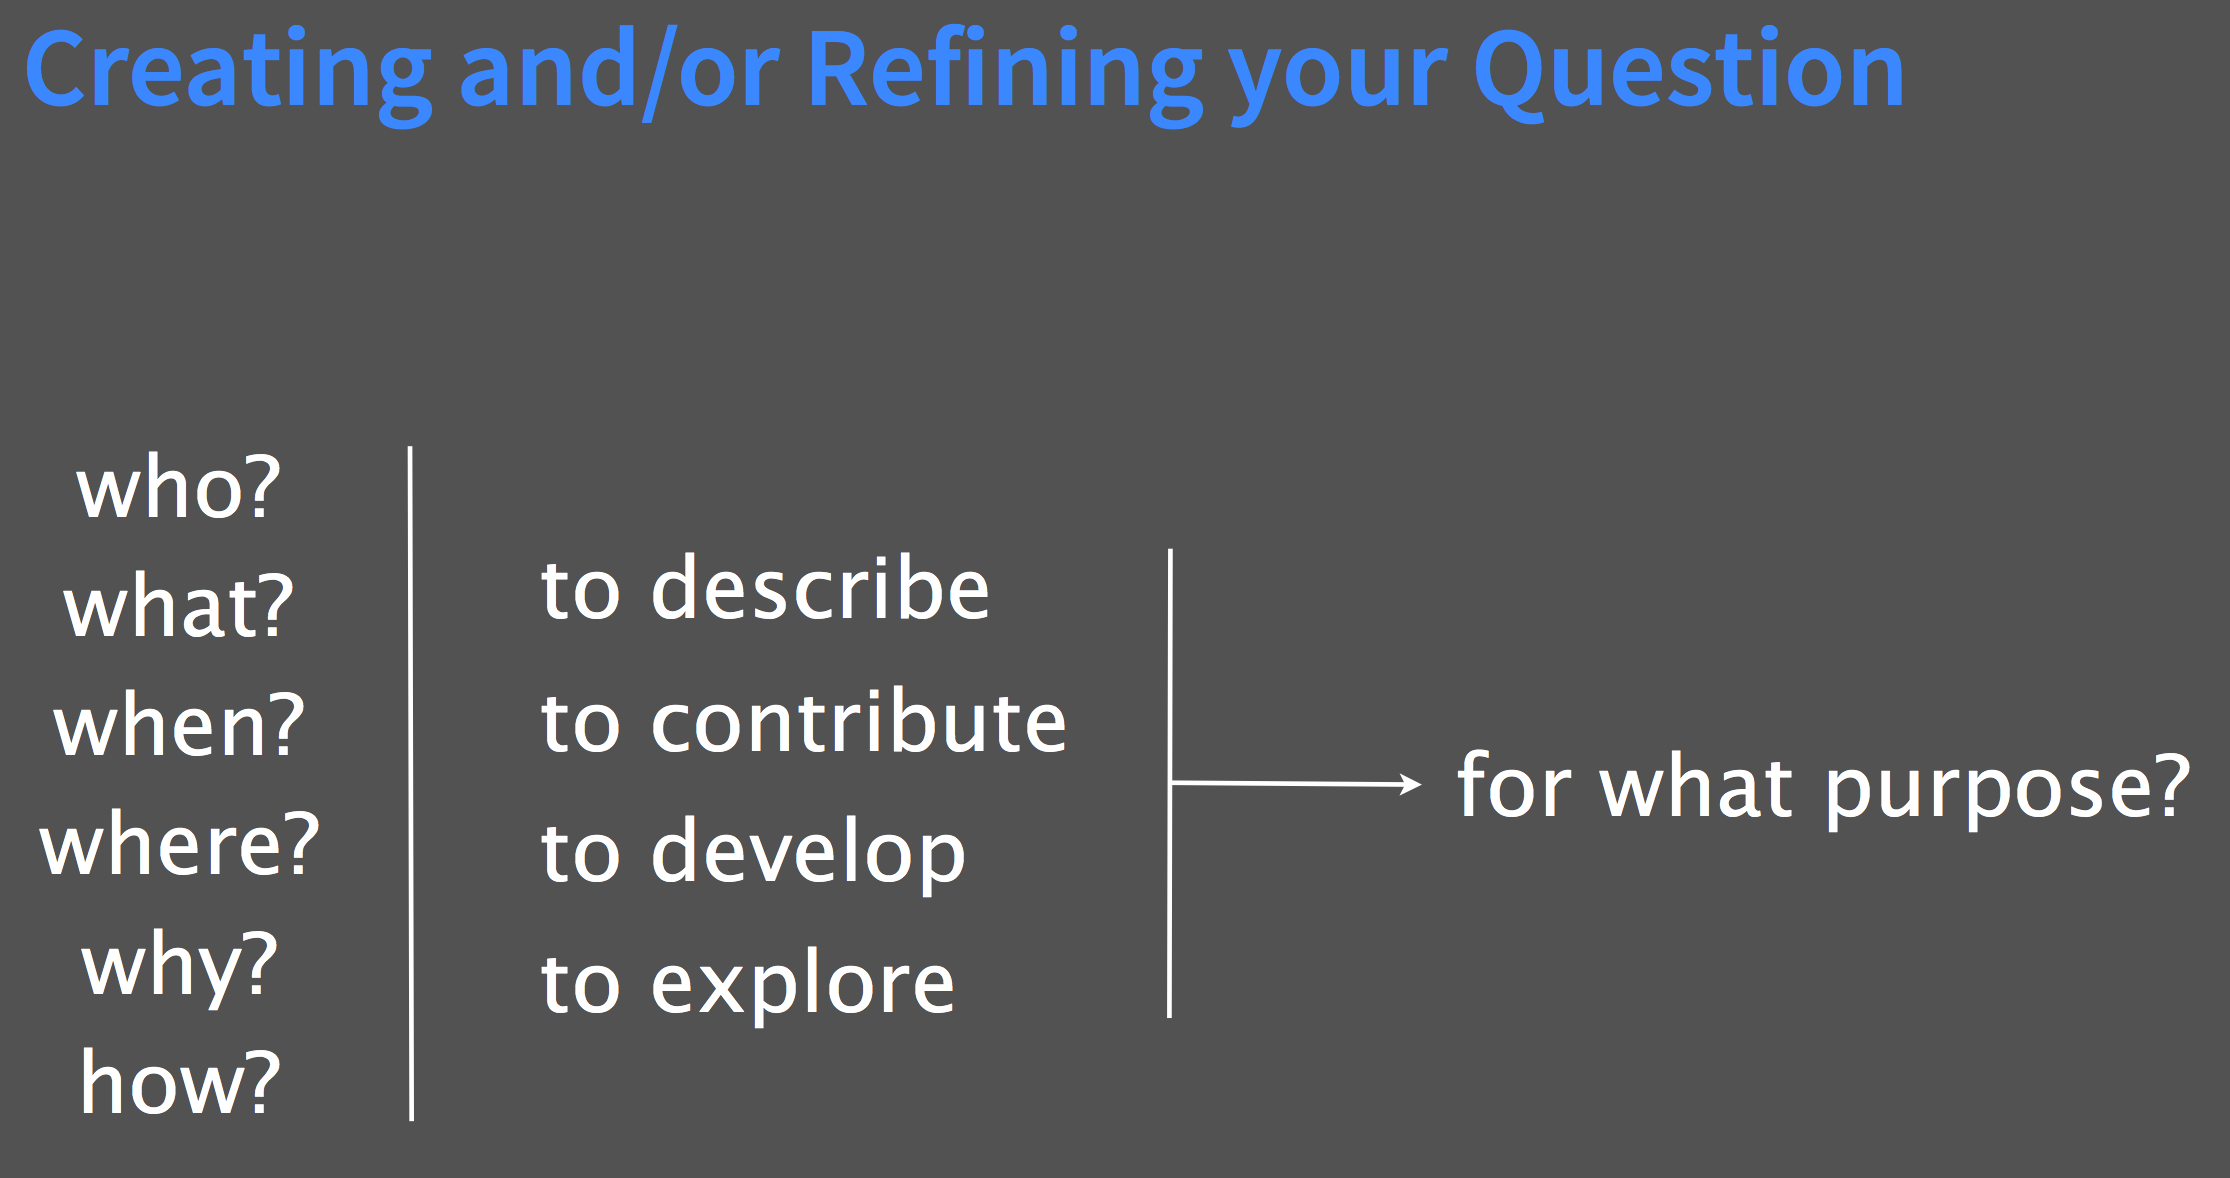
\includegraphics{images/creating-refinining-question.png}
\caption{Creating and/or refining your research question, per DevDH.org}
\end{figure}

Following Appleford and Guiliano, we can refine our question, or our
problem, or our provocation down to its essence in order to figure out
the next parts of the the process. Knowing exactly what kind of
question, problem, or provocation we're after, we then have a better
sense of what to do when confronted with a mass of data (for instance,
the excavation diaries from Kenen Tepe held in
\href{https://opencontext.org/projects/3DE4CD9C-259E-4C14-9B03-8B10454BA66E}{OpenContext.org,
deposited by Parker and Cobb, 2012}). Once the question is well-drawn
out, questions 3 and 4 take care of themselves.

One other element that we might add is `collaboration'. How do you plan
to collaborate? While many digital archaeology projects are done by a
single individual working in the quiet of their own space, most projects
require many different skill sets, perspectives, and stakeholders. It is
worth figuring out at the outset how you plan to work together. Will you
use email? Will you use a private \href{http://slack.com}{slack} or
messaging client? What about Kanban boards? (A Kanban board can be as
simple as a whiteboard with three columns on it, marked `to do',
`doing', and `done'. Tasks are written on post-it notes and moved
through the columns as necessary. A popular software implementation of a
Kanban board is \href{http://trello.com}{Trello}.) We would also
recommend that you write down the ideal division of labour and areas of
responsibility for each of the participants, \emph{along with a
mechanism for resolving disputes}.

Finally, how much time would you have to work on your digital
archaeology project? All of us have multiple demands on our time. Let's
be realistic about how much time you have available. How many hours,
total, do you spend in class, at work, asleep, and socializing? Add that
up for a week, then multiply by the number of weeks in your term. There
are 384 hours in a 16 week term. Subtract to find out how many `spare'
hours you can devote to homework, this project, or a hobbby.

Divide that by the number of weeks your course runs. That's how many
hours per week you can spend on all your non in-class course work. Then,
divide those hours by the number of courses you have.

That's how much time you have for your project. It's not an awful lot,
which means that the more energy you put into planning, the more
effective your labour is going to be.

\subsection{Take-aways}\label{take-aways}

\begin{itemize}
\tightlist
\item
  be explicit about how collaboration will be managed
\item
  be explicit about how your research goals intersect with your audience
\item
  be brutally honest about your time and guard it jealously
\end{itemize}

\subsection{exercises}\label{exercises-1}

\begin{enumerate}
\def\labelenumi{\arabic{enumi}.}
\tightlist
\item
  (to be refined) Open a new textfile in the Archaebox. Call it
  `initial-project-idea.md'. Using \texttt{\#} to indicate headings,
  sketch out a question, problem, or provocation of your own that occurs
  to you as you browse the Kenen Tepe materials housed at
  \href{https://opencontext.org/projects/3DE4CD9C-259E-4C14-9B03-8B10454BA66E}{OpenContext.org}.
  Save that file.
\item
  create a project management plan. (to be fleshed out in more detail) -
  maybe provide a link or copy of an actual project-management document
  and direct the students to annotate (read others' annotations),
  reflect on what the document does and where the trouble points are
  going to be?
\end{enumerate}

\hypertarget{github-version-control}{\section{Github \& Version
Control}\label{github-version-control}}

It's a familiar situation - you've been working on a paper. It's where
you want it to be, and you're certain you're done. You save it as
`final.doc'. Then, you ask your friend to take a look at it. She spots
several typos and that you flubbed an entire paragraph. You open it up,
make the changes, and save as `final-w-changes.doc'. Later that day it
occurs to you that you don't like those changes, and you go back to the
original `final.doc', make some changes, and just overwrite the previous
version. Soon, you have a folder like:

\begin{verbatim}
|-project
    |-'finalfinal.doc'
    |-'final-w-changes.doc'
    |-'final-w-changes2.doc'
    |-'isthisone-changes.doc'
    |-'this.doc'
\end{verbatim}

Things can get messy quite quickly. Imagine that you also have several
spreadsheets in there as well, images, snippets of code\ldots{} we don't
want this. What we want is a way of managing the evolution of your
files. We do this with a program called
\href{https://git-scm.com/}{Git}. Git is not a user-friendly piece of
software, and it takes some work to get your head around. Git is also
very powerful, but fortunately, the basic uses to which most of us put
it to are more or less straightforward. There are many other programs
that make use of Git for version control; these programs weld a
graphical user interface on top of the main Git program. It is better
however to become familiar with the basic uses of git from the command
line \emph{first} before learning the idiosyncracies of these helper
programs. The exercises in this section will take you through the basics
of using Git from the command line.

\subsection{The core functions of Git}\label{the-core-functions-of-git}

\begin{figure}[htbp]
\centering
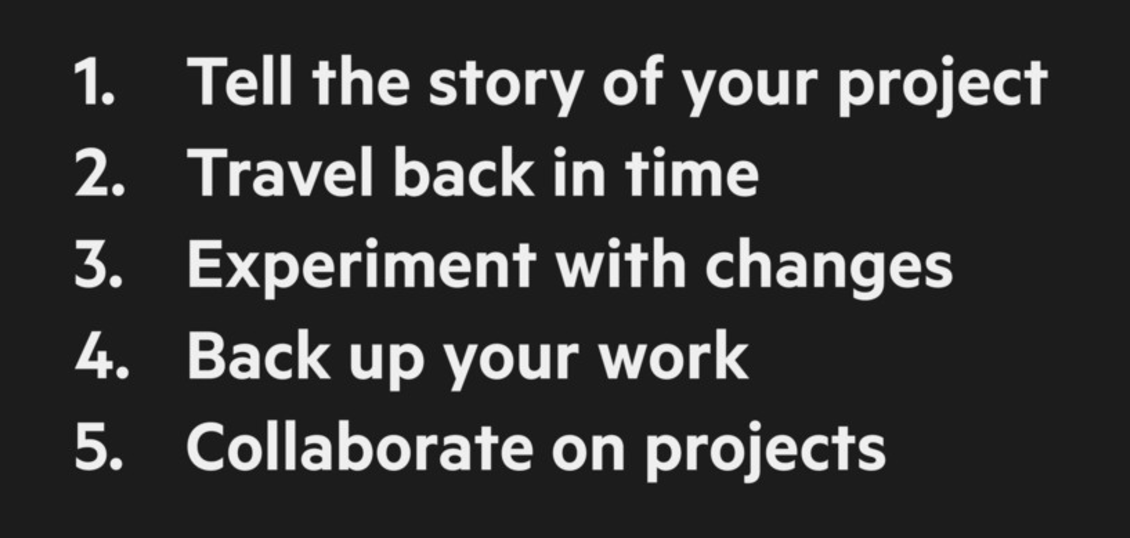
\includegraphics{images/what-git-does.png}
\caption{Alice Bartlett's summary of what Git does}
\end{figure}

At its heart, Git is a way of taking `snapshots' of the current state of
a folder, and saving those snapshots in sequence. (For an excellent
brief presentation on Git, see Alice Bartlett's
\href{https://speakerdeck.com/alicebartlett/git-for-humans}{presentation
here}; Bartlett is a senior developer for the Financial Times). In Git's
lingo, a folder on your computer is known as a \texttt{repository}. This
sequence of snapshots in total lets you see how your project unfolded
over time. Each time you wish to take a snapshot, you make a
\texttt{commit}. A commit is a Git command to take a snapshot of the
entire repository. Thus, your folder we discussed above, with its
proliferation of documents becomes:

\begin{verbatim}
|-project
    |-'final.doc'
\end{verbatim}

BUT its commit history could be visualized like this:

\begin{figure}[htbp]
\centering

\includegraphics{images/commit-history.png}
\caption{A visualization of the history of commits}
\end{figure}

Each one of those circles represents a point in time when you the writer
made a commit; Git compared the state of the file to the earlier state,
and saved a snapshot of the \texttt{differences}. What is particularly
useful about making a commit is that Git requires two more pieces of
information about the git: who is making it, and when. The final useful
bit about a commit is that you can save a detailed message about
\emph{why} the commit is being made. In our hypothetical situation, your
first commit message might look like this:

\begin{verbatim}
Fixed conclusion

Julie pointed out that I had missed 
the critical bit in the assignment 
regarding stratigraphy. This was 
added in the concluding section.
\end{verbatim}

This information is stored in the history of the commits. In this way,
you can see exactly how the project evolved and why. Each one of these
commits has what is called a \texttt{hash}. This is a unique fingerprint
that you can use to `time travel' (in Bartlett's felicitous phrasing).
If you want to see what your project looked like a few months ago, you
\texttt{checkout} that commit. This has the effect of `rewinding' the
project. Once you've checked out a commit, don't be alarmed when you
look at the folder: your folder (your repository) looks like how it once
did all those weeks ago! Any files written after that commit seem as if
they've disappeared. Don't worry: they still exist!

What would happen if you wanted to experiment or take your project in a
new direction from that point forward? Git lets you do this. What you
will do is create a new \texttt{branch} of your project from that point.
You can think of a branch as like the branch of a tree, or perhaps
better, a branch of a river that eventually merges back to the source.
(Another way of thinking about branches is that it is a label that
sticks with these particular commits.) It is generally considered `best
practice' to leave your \texttt{master} branch alone, in the sense that
it represents the best version of your project. When you want to
experiment or do something new, you create a \texttt{branch} and work
there. If the work on the branch ultimately proves fruitless, you can
discard it. \emph{But}, if you decide that you like how it's going, you
can \texttt{merge} that branch back into your master. A merge is a
commit that folds all of the commits from the branch with the commits
from the master.

Git is also a powerful tool for backing up your work. You can work quite
happily with Git on your own machine, but when you store those files and
the history of commits somewhere remote, you open up the possibility of
collaboration \emph{and} a safe place where your materials can be
recalled if -perish the thought- something happened to your computer. In
Git-speak, the remote location is, well, the \texttt{remote}. There are
many different places on the web that can function as a remote for Git
repositories. You can even set one up on your own server, if you want.
One of the most popular (and the one that we use for ODATE) is
\href{http://github.com}{Github}. There are many useful repositories
shared via Github of interest to archaeologists -
\href{http://opencontext.org}{OpenContext} for instance shares a lot of
material that way. To get material \emph{out} of Github and onto your
own computer, you \texttt{clone} it. If that hypothetical paper you were
writing was part of a group project, your partners could clone it from
your Github space, and work on it as well!

You and Anna are working together on the project. You have made a new
project repository in your Github space, and you have cloned it to your
computer. Anna has cloned it to hers. Let's assume that you have a very
productive weekend and you make some real headway on the project. You
\texttt{commit} your changes, and then \texttt{push} them from your
computer to the Github version of your repository. That repository is
now one commit \emph{ahead} of Anna's version. Anna \texttt{pulls} those
changes from Github to her own version of the repository, which now
looks \emph{exactly} like your version. What happens if you make changes
to the exact same part of the exact same file? This is called a
\texttt{conflict}. Git will make a version of the file that contains
text clearly marking off the part of the file where the conflict occurs,
with the conflicting information marked out as well. The way to
\texttt{resolve} the conflict is to open the file (typically with a text
editor) and to delete the added Git text, making a decision on which
information is the correct information.

\subsection{Key Terms}\label{key-terms}

\begin{itemize}
\tightlist
\item
  repository: a single folder that holds all of the files and subfolders
  of your project
\item
  commit: this means, `take a snapshot of the current state of my
  repostiory'
\item
  publish: take my folder on my computer, and copy it and its contents
  to the web as a repository at github.com/myusername/repositoryname
\item
  sync: update the web repository with the latest commit from my local
  folder
\item
  branch: make a copy of my repository with a `working name'
\item
  merge: fold the changes I have made on a branch into another branch
\item
  fork: to make a copy of someone else's repo
\item
  clone: to copy an online repo onto your own computer
\item
  pull request: to ask the original maker of a repo to `pull' your
  changes into their master, original, repository
\item
  push: to move your changes from your computer to the online repo
\item
  conflict: when two commits describe different changes to the same part
  of a file
\end{itemize}

\subsection{Take-aways}\label{take-aways-1}

\begin{itemize}
\tightlist
\item
  Git keeps track of all of the differences in your files, when you take
  a `snapshot' of the state of your folder (repository) with the
  \texttt{commit} command
\item
  Git allows you to roll back changes
\item
  Git allows you to experiment by making changes that can be deleted or
  incorporated as desired
\item
  Git allows you to manage collaboration safely
\item
  Git allows you to distribute your materials
\end{itemize}

\subsection{Further Reading}\label{further-reading}

We alluded above to the presence of `helper' programs that are designed
to make it easier to use Git to its full potential. An excellent
introduction to Github's desktop GUI is at this
\href{http://programminghistorian.org/lessons/getting-started-with-github-desktop}{Programming
Historian lesson on Github}. A follow-up lesson explains the way Github
itself can be used to host entire websites! You may explore it
\href{http://programminghistorian.org/lessons/building-static-sites-with-jekyll-github-pages}{here}.
In the section of this chapter on open notebooks, we will also use Git
and Github to create a simple open notebook for your research projects.

You might also wish to dip into the
\href{https://www.youtube.com/watch?v=D0_j04BnVeA}{archived live stream;
link here} from the first day of the NEH funded Institute on Digital
Archaeology Method and Practice (2015) where Prof.~Ethan Watrall
discusses project management fundamentals and, towards the last part of
the stream, introduces Git.

\subsection{Exercises}\label{exercises-2}

\begin{enumerate}
\def\labelenumi{\arabic{enumi}.}
\tightlist
\item
  How do you turn a folder into a repository? With the
  \texttt{git\ init} command. At the command line (remember, the
  \texttt{\$} just shows you the prompt; you don't have to type it!):
\end{enumerate}

\begin{enumerate}
\def\labelenumi{\alph{enumi}.}
\tightlist
\item
  make a new director: \texttt{\$\ mkdir\ first-repo}
\item
  type \texttt{\$\ ls} (list) to see that the director exists. Then
  change directory into it: \texttt{cd\ first-repo}. (remember: if
  you're ever not sure what directory you're in, type \texttt{\$\ pwd},
  or print working directory).
\item
  make a new file called \texttt{readme.md}. You do this by calling the
  text editor: \texttt{nano\ readme.md}. Type an explanation of what
  this exercise is about. The \texttt{.md} signals that you're writing a
  text file that uses the markdown format of signalling things like
  headings, lists, tables, etc. (A guide to
  \href{https://daringfireball.net/projects/markdown/basics.php}{markdown
  syntax is here}). Hit ctrl+x to exit, then y to save, leave the file
  name as it is.
\item
  type \texttt{\$\ ls} again to check that the file is there.
\item
  type \texttt{\$\ git\ init} to tell the Git program that this folder
  is to be tracked as a repository. If all goes correctly, you should
  see a variation on this message:
  \texttt{Initialized\ empty\ Git\ repository\ in\ /home/demonstration/first-repo/.git/}.
  But type \texttt{\$\ ls} again. What do you (not) see?
\end{enumerate}

The changes in your repo will now be stored in that \emph{hidden}
directory, \texttt{.git}. Most of the time, you will never have reason
to search that folder out. But know that the config file that describes
your repo is in that folder. There might come a time in the future where
you want to alter some of the default behaviour of the git program. You
do that by opening the config file (which you can read with a text
editor). Google `show hidden files and folders' for your operating
system when that time comes.

\begin{enumerate}
\def\labelenumi{\arabic{enumi}.}
\setcounter{enumi}{1}
\tightlist
\item
  Open your readme.md file again with the nano text editor, from the
  command line. Add some more information to it, then save and exit the
  text editor.
\end{enumerate}

\begin{enumerate}
\def\labelenumi{\alph{enumi}.}
\tightlist
\item
  type \texttt{\$\ git\ status}
\item
  Git will respond with a couple of pieces of information. It will tell
  you which \texttt{branch} you are on. It will list any untracked files
  present or new changes that are unstaged. We now will \texttt{stage}
  those changes to be added to our commit history by typing
  \texttt{\$\ git\ add\ -A}. (the bit that says \texttt{-A} adds any
  new, modified, or deleted files to your commit when you make it. There
  are
  \href{https://stackoverflow.com/questions/572549/difference-between-git-add-a-and-git-add\#572660}{other
  options or flags} where you add \emph{only} the new and modified
  files, \emph{or} only the modified and deleted files.)
\item
  Let's check our git status again: type \texttt{\$\ git\ status}
\item
  You should see something like this:
\end{enumerate}

\begin{verbatim}
On branch master
Initial commit
Changes to be committed:
  (use "git rm --cached <file>..." to unstage)
        new file:   readme.md```
\end{verbatim}

\begin{enumerate}
\def\labelenumi{\alph{enumi}.}
\setcounter{enumi}{4}
\tightlist
\item
  Let's take a snapshot: type
  \texttt{\$\ git\ commit\ -m\ "My\ first\ commit"}. What happened?
  Remember, Git keeps track not only of the changes, but \emph{who} is
  making them. If this is your first time working with Git in the
  Archaebox, Git will ask you for your name and email. Helpfully, the
  Git error message tells you exactly what to do: type
  \texttt{\$\ git\ config\ -\/-global\ user.email\ "you\textbackslash{}@example.com"}
  and then type
  \texttt{\$\ git\ config\ -\/-global\ user.name\ "Your\ Name"}. Now try
  making your first commit.
\item
  The command above represents a bit of a shortcut for making commit
  messages by using the \texttt{-m} flag to associate the text in the
  quotation marks with the commit. Open up your readme.md file again,
  and add some more text to it. Save and exit the text editor. Add the
  new changes to the snapshot that we will take. Then, type
  \texttt{\$\ git\ commit}. Git automatically opens up the text editor
  so you can type a longer, more substantive commit message. In this
  message (unlike in markdown) the \texttt{\#} indicates a line to be
  ignored. You'll see that there is already some default text in there
  telling you what to do. Type a message indicating the nature of the
  changes you have made. Then save and exit the text editor. DO NOT
  change the filename!
\end{enumerate}

Congratulations, you are now able to track your changes, and keep your
materials under version control!

\begin{enumerate}
\def\labelenumi{\arabic{enumi}.}
\setcounter{enumi}{2}
\tightlist
\item
  Go ahead and make some more changes to your repository. Add some new
  files. Commit your changes after each new file is created. Now we're
  going to view the history of your commits. Type \texttt{\$\ git\ log}.
  What do you notice about this list of changes? Look at the time
  stamps. You'll see that the entries are listed in reverse
  chronological order. Each entry has its own `hash' or unique ID, the
  person who made the commit and time are listed, as well as the commit
  message eg:
\end{enumerate}

\begin{verbatim}
commit 253506bc23070753c123accbe7c495af0e8b5a43
Author: Shawn Graham <shawn.graham@carleton.ca>
Date:   Tue Feb 14 18:42:31 2017 +0000

Fixed the headings that were broken in the about section of readme.md
\end{verbatim}

\begin{enumerate}
\def\labelenumi{\alph{enumi}.}
\tightlist
\item
  We're going to go back in time and create a new branch. You can escape
  the \texttt{git\ log} by typing \texttt{q}. Here's how the command
  will look:
  \texttt{\$\ git\ checkout\ -b\ branchname\ \textless{}commit\textgreater{}}
  where \texttt{branch} is the name you want the branch to be called,
  and \texttt{\textless{}commit\textgreater{}} is that unique ID. Make a
  new branch from your second last commit (don't use \textless{} or
  \textgreater{}).
\item
  We typed
  \texttt{git\ checkout\ -b\ experiment\ 253506bc23070753c123accbe7c495af0e8b5a43}.
  The response:
  \texttt{Switched\ to\ a\ new\ branch\ \textquotesingle{}experiment\textquotesingle{}}
  Check git status and then list the contents of your repository. What
  do you see? You should notice that some of the files you had created
  before seem to have disappeared - congratulations, you've time
  travelled! Those files are not missing; but they \emph{are} on a
  different branch (the master branch) and you can't harm them now. Add
  a number of new files, making commits after each one. Check your git
  status, and check your git log as you go to make sure you're getting
  everything. Make sure there are no unstaged changes - everything's
  been committed.
\end{enumerate}

\begin{enumerate}
\def\labelenumi{\arabic{enumi}.}
\setcounter{enumi}{3}
\tightlist
\item
  Now let's assume that your \texttt{experiment} branch was successful -
  everything you did there you were happy with and you want to integrate
  all of those changes back into your \texttt{master} branch. We're
  going to merge things. To merge, we have to go back to the master
  branch: \texttt{\$\ git\ checkout\ master}. (Good practice is to keep
  separate branches for all major experiments or directions you go. In
  case you lose track of the names of the branches you've created, this
  command: \texttt{git\ branch\ -va} will list them for you.)
\end{enumerate}

\begin{enumerate}
\def\labelenumi{\alph{enumi}.}
\tightlist
\item
  Now, we merge with \texttt{\$\ git\ merge\ experiment}. Remember, a
  merge is a special kind of commit that rolls all previous commits from
  both branches into one - Git will open your text editor and prompt you
  to add a message (it will have a default message already there if you
  want it). Save and exit and ta da! Your changes have been merged
  together.
\end{enumerate}

\begin{enumerate}
\def\labelenumi{\arabic{enumi}.}
\setcounter{enumi}{4}
\tightlist
\item
  One of the most powerful aspects of using Git is the possibility of
  using it to manage collaborations. To do this, we have to make a copy
  of your repository available to others as a \texttt{remote}. There are
  a variety of places on the web where this can be done; one of the most
  popular at the moment is \href{http://github.com}{Github}. Github
  allows a user to have an unlimited number of \texttt{public}
  repositories. Public repositories can be viewed and copied by anyone.
  \texttt{Private} repositories require a paid account, and access is
  controlled. If you are working on sensitive materials that can only be
  shared amongst the collaborators on a project, you should invest in an
  upgraded account (note that you can also control which files get
  included in commit; see
  \href{https://help.github.com/articles/ignoring-files/}{this help
  file}. In essence, you simply list the file names you do not want
  committed; here's an
  \href{https://gist.github.com/octocat/9257657}{example}). Let's assume
  that your materials are not sensitive.
\end{enumerate}

\begin{enumerate}
\def\labelenumi{\alph{enumi}.}
\item
  Go to Github, register for an account.
\item
  On the upper right part of the screen there is a large + sign. Click
  on that, and select \texttt{new\ public\ repository}
\item
  On the following screen, give your repo a name.
\item
  DO NOT `initialize this repo with a readme.md'. Leave
  \texttt{add\ .gitignore} and \texttt{add\ license} set to NONE.
\item
  Clic the green `Create Repository' button.
\item
  You now have a space into which you will publish the repository on
  your machine. At the command line, we now need to tell Git the
  location of this space. We do that with the following command, where
  you will change \texttt{your-username} and \texttt{your-new-repo}
  appropriately:

\begin{verbatim}
$ git remote add origin https://github.com/YOUR-USERNAME/YOUR-NEW-REPO.git
\end{verbatim}
\item
  Now we push your local copy of the repository onto the web, to the
  Github version of your repo:

\begin{verbatim}
git push -u origin master
\end{verbatim}
\end{enumerate}

\emph{NB} If you wanted to push a \texttt{branch} to your repository on
the web instead, do you see how you would do that? If your branch was
called \texttt{experiment}, the command would look like this:

\begin{verbatim}
$ git push origin experiment
\end{verbatim}

\begin{enumerate}
\def\labelenumi{\alph{enumi}.}
\setcounter{enumi}{7}
\tightlist
\item
  The changes can sometimes take a few minutes to show up on the
  website. Now, the next time you make changes to this repository, you
  can push them to your Github account - which is the `origin' in the
  command above. Add a new text file. Commit the changes. Push the
  changes to your account.
\end{enumerate}

\begin{enumerate}
\def\labelenumi{\arabic{enumi}.}
\setcounter{enumi}{5}
\tightlist
\item
  Imagine you are collaborating with one of your classmates. Your
  classmate is in charge of the project, and is keeping track of the
  `official' folder of materials (eg, the repo). You wish to make some
  changes to the files in that repository. You can manage that
  collaboration via Github by making a copy, what Github calls a
  \texttt{fork}.
\end{enumerate}

\begin{enumerate}
\def\labelenumi{\alph{enumi}.}
\item
  Make sure you're logged into your Github account on the Github
  website. We're going to fork an example repository right now by going
  to \url{https://github.com/octocat/Spoon-Knife}. Click the `fork'
  button at top-right. Github now makes a copy of the repository in your
  own Github account!
\item
  To make a copy of that repository on your own machine, you will now
  clone it with the \texttt{git\ clone} command. (Remember: a `fork'
  copies someone's Github repo into a repo in your OWN Github account; a
  `clone' makes a copy on your own MACHINE). Type:

\begin{verbatim}
$ cd.. 
$ pwd
\end{verbatim}

  We do that to make sure you're not \emph{inside} any other repo you've
  made! Make sure you're not inside the repository we used in exercises
  1 to 5, then proceed:
\end{enumerate}

\begin{verbatim}
$ git clone https://github.com/YOUR-USERNAME/Spoon-Knife
$ ls
\end{verbatim}

You now have a folder called `Spoon-Knife' on your machine! Any changes
you make inside that folder can be tracked with commits. You can also
\texttt{git\ push\ -u\ origin\ master} when you're inside it, and the
changes will show up on your OWN copy (your fork) on Github.com. c. Make
a fork of, and then clone, one of your classmates' repositories. Create
a new branch. Add a new file to the repository on your machine, and then
push it to your fork on Github. Remember, your new file will appear on
the new branch you created, NOT the master branch.

\begin{enumerate}
\def\labelenumi{\arabic{enumi}.}
\setcounter{enumi}{6}
\tightlist
\item
  Now, you let your collaborator know that you've made a change that you
  want her to \texttt{merge} into the original repository. You do this
  by issuing a \texttt{pull\ request}. But first, we have to tell Git to
  keep an eye on that original repository, which we will call
  \texttt{upstream}. You do this by adding that repository's location
  like so:
\end{enumerate}

\begin{enumerate}
\def\labelenumi{\alph{enumi}.}
\tightlist
\item
  type (but change the address appropriately):
\end{enumerate}

\begin{verbatim}
$ git remote add upstream THE-FULL-URL-TO-THEIR-REPO-ENDING-WITH-.git
\end{verbatim}

\begin{enumerate}
\def\labelenumi{\alph{enumi}.}
\setcounter{enumi}{1}
\item
  You can keep your version of the remote up-to-date by fetching any new
  changes your classmate has done:

\begin{verbatim}
$ git fetch upstream
\end{verbatim}
\item
  Now let's make a \texttt{pull} request (you might want to bookmark
  this
  \href{https://help.github.com/articles/creating-a-pull-request/}{help
  document}). Go to your copy of your classmate's repository at your
  Github account. Make sure you've selected the correct branch you
  pushed your changes to, by selecting it from the Branches menu drop
  down list.
\item
  Click the `new pull request' button.
\item
  The new page that appears can be confusing, but it is trying to double
  check with you which changes you want to make, and where. \emph{`Base
  Branch'} is the branch where you want your changes to go, ie, your
  classmate's repository. \emph{`head branch'} is the branch where you
  made \emph{your} changes. Make sure these are set properly. Remember:
  the first one is the TO, the second one is the FROM: the place where
  you want your changes to go TO, FROM the place where you made the
  changes.
\item
  A pull request has to have a message attached to it, so that your
  classmate knows what kind of change you're proposing. Fill in the
  message fields appropriately, then hit the `create pull request'
  button.
\end{enumerate}

\begin{figure}[htbp]
\centering
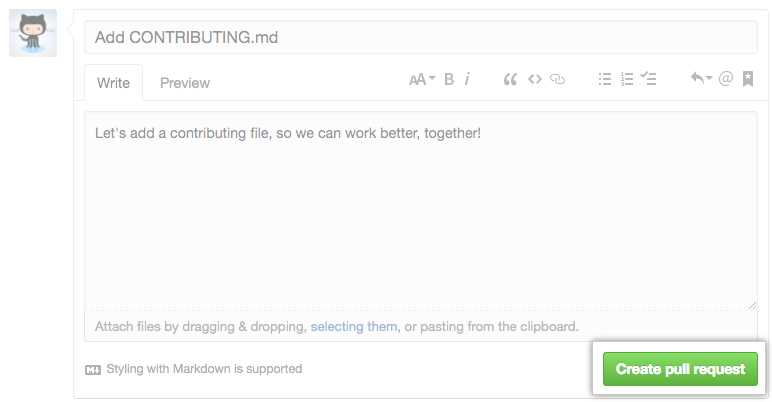
\includegraphics{images/pullrequest-send.png}
\caption{A pull request message; Image from Github.com}
\end{figure}

\begin{enumerate}
\def\labelenumi{\arabic{enumi}.}
\setcounter{enumi}{7}
\tightlist
\item
  Finally, the last bit of work to be done is to accept the pull request
  and \texttt{merge} the changes into the original repository.
\end{enumerate}

\begin{enumerate}
\def\labelenumi{\alph{enumi}.}
\item
  Go to your repository on your Github account. Check to see if there
  are any `pull requests' - these will be listed under the `pull
  requests' tab. Click on that tab.
\item
  You can merge from the command line, but for now, you can simply click
  on the green `merge pull request' button, and then the `confirm merge'
  button. The changes your classmate has made have now been folded into
  your repository.
\item
  To get the updates on your local machine, go back to the command line
  and type

\begin{verbatim}
$ git pull origin master
\end{verbatim}
\end{enumerate}

\subsection{Warnings}\label{warnings}

It is possible to make changes to files directly via the edit button on
Github. Be careful if you do this, because things rapidly can become out
of sync, resulting in conflicts between differing versions of the same
file. Get in the habit of making your changes on your own machine, and
making sure things are committed and up-to-date (\texttt{git\ status},
\texttt{git\ pull\ origin\ master}, \texttt{git\ fetch\ upstream} are
your friends) before beginning work. At this point, you might want to
investigate some of the graphical interfaces for Git (such as
\href{https://desktop.github.com/}{Github Desktop}). Knowing as you do
how things work from the command line, the idiosyncracies of the
graphical interfaces will make more sense. For further practice on the
ins-and-outs of Git and Github Desktop, we recommend trying
\href{https://github.com/jlord/git-it-electron/}{the Git-it app} by
Jessica Lord.

For help in resolving merge conflicts, see the
\href{https://help.github.com/articles/resolving-a-merge-conflict-using-the-command-line/}{Github
help documentation}. For a quick reminder of how the workflow should go,
see
\href{https://gist.github.com/shawngraham/513d4b2860d52fdac6bd783e4387957e}{this
cheat-sheet by Chase Pettit}.

\hypertarget{open-notebook-research-scholarly-communication}{\section{Open
Notebook Research \& Scholarly
Communication}\label{open-notebook-research-scholarly-communication}}

Digital archaeology necessarily generates a lot of files. Many of those
files are data; many more are manipulations of that data, or the data in
various stages of cleaning and analysis. Without any sort of version
control or revision history (as detailed in the previous section), these
files quickly replicate to the point where a project can be in serious
danger of failing. Which file contains the `correct' data? The correct
analysis? Even worse, imagine coming back to a project after a few
months' absence. Worse still, after a major operating system update of
the kind foisted on Windows users from Windows 7 to Windows 10. The bad
news continues: magnetic storage can fail; online cloud services can be
hacked; a key person on the project can die.

Even if the data makes it to publication, there is the problem of the
data not being available to others for re-interrogation or re-analysis.
Requests for data from the authors of journal articles are routinely
ignored, whether by accident or design. Researchers may sit on data for
years. We have all of us had the experience of working on a collection
of material, and then writing to the author of the original article,
requesting an explanation for some aspect of the data schema used, only
to find out that the author has either died, kept no notes, left the
field entirely, or simply doesn't remember.

There is no excuse for this any longer. \texttt{Open\ notebook\ science}
is a gathering movement across a number of fields to make the entire
research process transparent by sharing materials online as they are
generated. These include everything from the data files themselves, to
the code used to manipulated it, to notes and observations in various
archives. Variations on this `strong' position include data-publishing
of the materials after the main paper has been published (see for
instance \href{http://opencontext.org}{OpenContext} or the
\href{http://openarchaeologydata.metajnl.com/}{Journal of Open
Archadological Data}). Researchers such as
\href{https://faculty.washington.edu/bmarwick/}{Ben Marwick} and
\href{http://notebook.madsenlab.org/labnotebook.html}{Mark E. Madsen}
are leading the field in archaeology, while scholars such as
\href{http://wcm1.web.rice.edu/open-notebook-history.html}{Caleb
McDaniel} are pushing the boundaries in history. The combination of
simple text files (whether written text or tabular data such as .csv
files) with static website generators (ie, html rather than dynamically
generated database websites like Wordpress) enables the live publishing
of in-progress work.
\href{http://www.carlboettiger.info/2012/09/28/Welcome-to-my-lab-notebook.html}{Carl
Boettiger} is often cited as one of the godfathers of this movement. He
makes an important distinction:

\begin{quote}
This {[}notebook, not blog{]} is the active, permanent record of my
scientific research, standing in place of the traditional paper bound
lab notebook. The notebook is primarily a tool for me to do science, not
communicate it. I write my entries with the hope that they are
intelligible to my future self; and maybe my collaborators and experts
in my field. Only the occasional entry will be written for a more
general audience. {[}\ldots{}{]} In these pages you will find not only
thoughts and ideas, but references to the literature I read, the codes
or manuscripts I write, derivations I scribble and graphs I create and
mistakes I make. (Boettiger)
\end{quote}

Major funding bodies are starting to require a similar transparency in
the research that they support. Recently, the Social Sciences and
Humanities Research Council of Canada published guidance on
\href{http://www.sshrc-crsh.gc.ca/about-au_sujet/policies-politiques/statements-enonces/edata-donnees_electroniques-eng.aspx}{data
management plans}:

\begin{quote}
All research data collected with the use of SSHRC funds must be
preserved and made available for use by others within a reasonable
period of time. SSHRC considers ``a reasonable period'' to be within two
years of the completion of the research project for which the data was
collected.
\end{quote}

Annecdotally, we have also heard of work being denied funding because
the data management plan, and/or the plan for knowledge mobilization,
made only the briefest of nods towards these issues: `we shall have a
blog and will save the data onto a usb stick' does not cut it any more.
A recent volume of case-studies in `reproducible research' includes a
contribution from Ben Marwick that details not only the benefits of such
an approach, but also the `pain points'. Key amongst them was that not
everyone participating in the project was on board using scripted code
to perform the analysis (preferring instead to use the point-and-click
of Excel), the duplication of effort that emerged as a result, and the
complexities that arose from what he calls the `dual universes' of
Microsoft tools versus the open source tools. (MARWICK REF). On the
other hand, the advantages outweighed the pain. For Marwick's team,
because their results and analysis can be re-queried and
re-interrogated, they have an unusually high degree of confidence in
what they've produced. Their data, and their results have a complete
history of revisions that can be examined by reviewers. Their code can
be re-used and re-purposed, thus making their subsequent research more
efficient. Marwick goes on to create an entire `compendium' of code,
notes, data, and software dependencies that can be duplicated by other
researchers. Indeed, we will be re-visiting their compendium in Section
XXXXXXXXX.

Ultimately, McDaniels says it best about keeping open notebooks of
research in progress when he writes,

\begin{quote}
The truth is that we often don't realize the value of what we have until
someone else sees it. By inviting others to see our work in progress, we
also open new avenues of interpretation, uncover new linkages between
things we would otherwise have persisted in seeing as unconnected, and
create new opportunities for collaboration with fellow travelers. These
things might still happen through the sharing of our notebooks after
publication, but imagine how our publications might be enriched and
improved if we lifted our gems to the sunlight before we decided which
ones to set and which ones to discard? What new flashes in the pan might
we find if we sifted through our sources in the company of others?
\end{quote}

A parallel development is the growing practice of placing materials
online as pre-prints or even as drafts, for sharing and for soliciting
comments. Graham for instance uses a blog as a place to share
longer-form discursive writing in progress; with his collaborators Ian
Milligan and Scott Weingart, he even wrote a book `live' on the web,
warts and all (which you may still view at
\href{http://themacroscope.org}{The Macroscope}). Sharing the draft in
progress allowed them to identify errors and ommissions as they wrote,
and for their individual chapters and sections to be incorporated into
class syllabi right away. In their particular case, they came to an
arrangment with their publisher to permit the draft to remain online
even after the formal publication of the `finished' book - which was
fortunate, as they ended up writing another chapter immediately after
publication! In this, they were building on the work of scholars such as
Kathleen Fitzpatrick, whose
\href{http://mcpress.media-commons.org/plannedobsolescence/}{\emph{Planned
Obsolescence}} was one of the first to use the Media Commons `comment
press' website to support the writing. Commentpress is a plugin for the
widely used Wordpress blogging system, which allows comments to be made
at the level of individual paragraphs. This textbook you are currently
reading uses another solution, the
\href{http://hypothes.is}{hypothes.is} plugin that fosters communal
reading and annotation of electronic texts. This points to another happy
by-product of sharing one's work this way - the ability to generate
communities of interest around one's research. The Kitz et al. volume is
written with the \href{http://gitbook.com}{Gitbook} platform, which is a
graphical interface for writing using Git at its core with markdown text
files to manage the collaboration. The commit history for the book then
also is a record of how the book evolved, and who did what to it when.
In a way, it functions a bit like `track changes' in Word, with the
significant difference that the evolution of the book can be rewound and
taken down different branches when desired.

In an ideal world, we would recommend that everyone should push for such
radical transparency in their research and teaching. But what is safe
for a group of (mostly) white, tenured, men is not safe for everyone
online. In which case, what we recommend is for individuals to assess
what is safest for them to do, while still making use of the affordances
of Git, remote repositories, and simple text files.
\href{http://bitbucket.org}{Bitbucket} at the time of writing offers
free private repositories (so you can push your changes to a remote
repository without fear of others looking or cloning your materials);
\href{http://reclaimhosting.com}{ReclaimHosting} supports academic
webhosting and allows one to set up the private `dropbox' like
file-sharing service \href{https://owncloud.org/}{Owncloud}.

In this exercises below, we will explore how to make a simple open
notebook via a combination of markdown files and a repository on Github.
Ultimately, we endorse the model developed by Ben Marwick, of creating
an entire `research compendium' that can be installed on another
researcher's machine, but a good place to start are with the historian
Lincoln Mullen's simple notebook templates. This will introduce to you
another tool in the digital archaeologist's toolkit, the open source R
programming language and the R Studio `IDE' ('integrated development
environment).

Far more complicated notebooks are possible, inasmuch as they combine
more features and ways of compiling your research. Scholars such as
\href{http://notebook.madsenlab.org/}{Mark Madsen} use a combination of
Github pages and the Jekyll blog generator (for more on using Jekyll to
create static websites, see Amanda Visconti's
\href{http://programminghistorian.org/lessons/building-static-sites-with-jekyll-github-pages}{Programming
Historian tutorial}.) A simple Github repository and Wordpress blog can
be used in tandem, where the blog serves for the \emph{narrative} part
of a notebook, the part that tries to make sense of the notes contained
in the repository. This aspect of open notebook science is critically
important in that it serves to signal your \emph{bona fides} as a
serious scholarly person. Research made available online is
\emph{findable}; given the way web search works, if something cannot be
found easily, it might as well not exist.

Ultimately, tou will need to work out what combination of tools works
best for you. Some of our students have had success using
\href{https://www.literatureandlatte.com/scrivener.php}{Scrivener} as a
way of keeping notes, where Scrivener writes to a repository folder or
some other folder synced across the web (like Dropbox, for instance). In
this workflow, you have one Scrivener file per project. Scrivener uses
the visual conceit of actual 3 x 5 notecards. Within Scrivener, one
would make one card per note, and keep them in a `research' folder.
Then, when it becomes time to write up the project, those notecards can
be moved into the draft and rearranged as necessary so that the writing
flows naturally from them.

\subsection{How to Ask Questions}\label{how-to-ask-questions}

\begin{itemize}
\tightlist
\item
  stuff here on how to ask a question on sites like stackoverflow etc.
\item
  also this
  \url{https://speakerdeck.com/jennybc/reprex-help-me-help-you},
  although perhaps move it to 3.1 literate programming. perhaps use it
  to create actual examples that can be copied over to R though. In
  which case, talk about it in both places.
\item
  the idea being ways in which your open notebook becomes an invitation
  to others to help you, and also, a way of making sure you find the
  answer you're looking for when the inevitable troubles emerge
\end{itemize}

\subsection{discussion}\label{discussion}

Questions for discussion:

\begin{enumerate}
\def\labelenumi{\arabic{enumi}.}
\tightlist
\item
  Search the archaeological literature (via
  \href{http://jstor.org}{jstor} or
  \href{https://scholar.google.ca/}{Google Scholar}) for examples of
  open notebook science `in the wild'. Are you finding anything, and if
  so, where? Do there seem to be impediments \emph{from the journals}
  regarding this practice?
\item
  What excites you about the possibilities of open notebook archaeology?
  What are the advantages?
\item
  What frightens you? What are the disadvantages?
\item
  Search online for the `replicability crisis in science'. Is there any
  such thing in archaeology?
\item
  Study Marwick's paper REF and compare it to its supporting Github
  repository. What \emph{new} questions could be asked of this data?
\item
  In what ways are terms like `open access', `open source', and `open
  science' synonyms for a similar approach, and in what ways are they
  different?
\end{enumerate}

\subsection{Take-aways}\label{take-aways-2}

Keeping an open notebook (or if necessary, a closed notebook) is a habit
that must be cultivated. As a target to aim for, try to have

\begin{itemize}
\tightlist
\item
  each experiment\textbar{}project in its own folder
\item
  each experiment\textbar{}project with regular pattern of subfolders
  \texttt{data} and \texttt{figures} and \texttt{text} and \texttt{bib}
  etc
\item
  the experiments\textbar{}projects under version control.
\item
  a plan for data publishing. One option is to submit the repository to
  \href{http://zenodo.org}{zenodo} or similar to obtain digital object
  identifiers (DOIs) for the repository
\item
  a plan to write as you go, on a fail log or blog or what-have-you.
  Obtain a DOI for this, too.
\end{itemize}

We haven't mentioned DOIs in this section, but when your notebook and
your narrative about your research has a DOI, it becomes easier for your
colleagues to cite your work - even this work in progress!

\subsection{Further Reading}\label{further-reading-1}

Baker, James. `Preserving Your Research Data', \emph{The Programming
Historian}
\url{http://programminghistorian.org/lessons/preserving-your-research-data}

\subsection{On Privilege and Open
Notebooks}\label{on-privilege-and-open-notebooks}

While we argue for open notebooks, there may be circumstances where this
is not desireable or safe to do. Readers may also want to explore an
Evernote alternative, \href{https://laverna.cc/}{Laverna} which stores
your notes in your web-browser's cache hence making them private, but
also allows sync to services such as Dropbox (versioning and backup are
still absolutely critical). If you work primarily on a Mac computer,
\href{http://brettterpstra.com/projects/nvalt/}{nvAlt by Brett Terpstra}
is an excellent note-taking application that can sync remotely. Another
possibility is \href{http://classeur.io/}{Classeur} a web abb that
integrates with various blogging platforms, allows for syncing and
collaboration, the choice of what to make public and what to keep
private, and includes the ability to sort notes into various notebooks.
It does \emph{not} save locally, so be warned that your information is
on their servers. There is an API (application programming interface)
that allows you to download your materials (for more on APIs, see
\protect\hyperlink{introduction-to-digital-libraries-archives-repositories}{Introduction
to Digital Libraries, Archives \& Repositories}).

A final word on the privilege involved in keeping an open notebook is
warranted. To make one's research available openly on the web, to
discuss openly the things that worked, the things that haven't, the
experiments tried and the dead ends explored, is at the current moment
something that depends on the perceived race, class, and gender of the
person doing it. What passes without comment when I (Shawn Graham, a
white, tenured, professor) do something could attract unwarranted,
unwanted, and unfair attention if a woman of colour undergraduate tried.
This is not to say this always happens; but disgracefully it happens far
too often. It is important and necessary to fight back against the
so-called `internet culture' in these things, but it is not worth
risking one's safety. To those who benefit from privilege, it is
incumbent upon them to make things safe for others, to recognize that
open science, open humanities, represents a net boon to our field. In
which case, it is up to them to normalize such practices, to make it
safe to try things out. We discuss more in the following section on what
\protect\hyperlink{failing-productively}{Failing Productively} means,
why it matters, and why it is integral not only to digital archaeology,
but the culture of academic research, teaching, and outreach more
generally.

\subsection{exercises}\label{exercises-3}

In this series of exercises, we are going to take you through the
process of setting up an open research notebook, where you control all
of the code and all of the data. A good rule-of-thumb in terms of
keeping a notebook is `one notecard per thought`, here adapted as 'one
file per thought, one folder per project'.

\begin{enumerate}
\def\labelenumi{\arabic{enumi}.}
\tightlist
\item
  Let us set up a template open-notebook based on
  \href{https://github.com/lmullen/rmd-notebook}{Lincoln Mullen's Simple
  RmD Notebook}. If you go to
  \url{https://lmullen.github.io/rmd-notebook/} you'll see a `live'
  version of this template on the web. It is being served to us from a
  special branch in Mullen's Github account, called \texttt{gh-pages}.
  When you have a \texttt{gh-branches} branch in very nearly any repo
  associated with your own Github account, Github.com will treat that
  repository \emph{not} as a repository but as an actual website. This
  allows us to update or experiment with changes on other branches, and
  show a `polished' version to the world via the \texttt{gh-pages}
  branch. That branch will have a special address, in the form
  \texttt{your-account-name.github.io/your-repo}. Whenever you see
  \texttt{github.io} in a URL, you know that the source for that website
  will be found at \texttt{github.com/account-name/repo}. Do you see the
  difference? (For more on \texttt{gh-pages}, see the
  \href{https://pages.github.com/}{Github documentation}).
\end{enumerate}

\begin{enumerate}
\def\labelenumi{\alph{enumi}.}
\item
  Begin sketching out on paper an idea for a digital archaeological
  project, perhaps the one you imagined at the end of our section on
  \protect\hyperlink{project-management-basics}{Project Management
  Basics}. Imagine its file structure. In the top level folder are going
  to go all of your notecards. Sub-folders are going to hold diagrams
  that you create in the course of your reserch; source-data that you
  leave untouched; data that you've cleaned or manipulated; any helper
  code that you might create; and so on. You will use this structure to
  help organize your open notebook once we've installed it.
\item
  Make a fork of our copy of Mullen's notebook (we've added
  \href{http://hypothes.is}{hypothes.is} to it). You can find our copy
  at \url{https://github.com/o-date/rmd-notebook}.
\item
  \texttt{Clone} your copy to the ODATE environment at the command line.
  (Review \protect\hyperlink{github-version-control}{Github \& Version
  Control} if necessary first).
\item
  Type \texttt{ls} to make sure the \texttt{rmd-notebook} directory is
  present; then \texttt{cd\ rmd-notebook}.
\item
  Check which branch you are on, and make sure it is the
  \texttt{gh-pages} branch. (Hint: check the status)
\item
  Now you're ready to start adding notes! Remember, \texttt{.Rmd} files
  are just markdown files into which you can insert working R code.
  We're not ready to do that yet (but we will
  \href{Statistical\%20Computing\%20with\%20R\%20and\%20Python\%20Notebooks;\%20Reproducible\%20code}{encounter
  it in due course}), but for now, you can think of these files as
  simple notecards where one card = one idea. Note the existing
  \texttt{.rmd} files in this folder. Their filenames all begin with a
  number. Yours should be numbered as well. You can create a new card by
  typing \texttt{nano\ filename.rmd} where \texttt{filename} is whatever
  you want it to be. Your notecard can include images by using the
  markdown syntax,
  \texttt{!{[}image\ tile{]}(path/to/image/filename.jpg)}; those images
  can be on the web or in an image folder. (A good place to practice
  markdown is at \href{http://dillinger.io}{Dillinger.io}).
\end{enumerate}

Your note \emph{must} contain some descriptive metadata at the top. This
is good practice no matter what kind of note-taking system you use. In
our case here, we use the \texttt{yaml} approach. This is what a minimum
example looks like:

\begin{verbatim}
---
title: "First page of the notebook"
author: "Lincoln Mullen"
date: "December 3, 2015"
---
\end{verbatim}

Title, author, and date. These will get passed to the
\texttt{\textless{}meta\textgreater{}} tags in the eventual HTML we are
going to generate. This information makes your site easier to find and
to archive and to associate with you as a scholar.

\begin{enumerate}
\def\labelenumi{\alph{enumi}.}
\setcounter{enumi}{6}
\tightlist
\item
  Now we make the public-facing website for your notebook. Mullen has
  bundled a series of commands into a \texttt{make} file, which acts as
  a short-cut for us and also ensures that the same sequence of
  operations is carried out everytime. (You can read more about
  makefiles \href{https://bost.ocks.org/mike/make/}{here}.) At the
  command prompt type \texttt{\$\ make}.
\end{enumerate}

\begin{verbatim}
SG <- note pandoc and rmarkdown have to be bundled into the box before hand. Otherwise, the following commands have to be run:
$ wget https://github.com/jgm/pandoc/releases/download/1.19.2.1/pandoc-1.19.2.1-1-amd64.deb
to get pandoc and then $ sudo dpkg -i pandoc-1.19.2.1-1-amd64.deb` to unzip and install it. Rmarkdown has to be installed from the R Server code pane. The first sample rmd file has a leaflet webapp in it; I modified the R to install leaflet first, but I dunno. This'll have to be tested. Probably easier at this point to just remove it.
\end{verbatim}

\begin{enumerate}
\def\labelenumi{\alph{enumi}.}
\setcounter{enumi}{7}
\tightlist
\item
  The make file is pushing all of your \texttt{.Rmd} files through a
  program called \texttt{pandoc}, and adding various styling options to
  make an entire website.
\end{enumerate}

\begin{quote}
As an aside, Pandoc is an extremely useful piece of software for
converting files from one format to another. A series of examples can be
found at \url{http://www.pandoc.org/demos.html}. At the command line,
type \texttt{\$\ pandoc} and then your source file, then indicate the
kind of output you want using the \texttt{-o} flag, eg:
\texttt{\$\ pandoc\ MANUAL.txt\ -o\ example1.html}. One of the outputs
Pandoc can generate is a Word document - which means, your source text
is kept in a very simple, future-proof format, and Word can be used just
for typography.
\end{quote}

Commit your changes and push them to your remote repository. Visit the
\texttt{live} version of your repository - ie, the one at
\texttt{github.io} \emph{not} \texttt{github.com} to see your live open
research notebook!

\begin{enumerate}
\def\labelenumi{\roman{enumi}.}
\tightlist
\item
  Write a new note for your notebook recording your work, the problems
  you encountered, and the solutions you found. Save, \texttt{make},
  commit, and push your note to the web.
\end{enumerate}

\begin{enumerate}
\def\labelenumi{\arabic{enumi}.}
\setcounter{enumi}{1}
\tightlist
\item
  Another approach involves writing markdown files, putting them online,
  and then using a kind of `helper' file to manage their display as
  html. In this particular case, we are going to use something called
  \texttt{mdwiki}.
  \href{https://dynalon.github.io/mdwiki/\#!index.md}{Mdwiki} involves a
  single html file which, when put in the same folder as a series of
  markdown files, acts as a kind of wrapper to turn the markdown files
  into pages of a wiki-style website. There is a lot of customization
  possible, but for now we're going to make a basic notebook out of a
  mdwiki template.
\end{enumerate}

\begin{enumerate}
\def\labelenumi{\alph{enumi}.}
\item
  Fork the minimal mdwiki template to your Github account;
  \href{https://github.com/exalted/mdwiki-seed}{md wiki template is
  linked here}
\item
  At this point, any markdown file you create and save into the
  \texttt{mdwiki-seed\textbackslash{}ll\_CC\textbackslash{}} folder will
  become a webpage, although \emph{the .md extension should still be
  used in the URL} . If you study the folder structure, you'll see that
  there are pre-made folders for pages, for pdfs, for images, and so on
  (if you clone the repo, you can then add or remove these folders as
  you like using the file manager). Remembering to frame any internal
  links as relative links. That is to say, if you saved a markdown file
  in \texttt{ll\_CC/pages/observation1.md} but wanted to link to
  \texttt{ll\_CC/pages/observation2.md}, it is enough to just add
  \texttt{{[}Click\ here{]}(observation2.md)}. Because the
  \texttt{mdwiki-seed} you forked was \emph{already} on a
  \texttt{gh-pages} branch, your notebook will be visible at
  \texttt{YOURUSERNAME.github.io/mdwiki-seed/}. But note: the page will
  reload and you'll see \texttt{\#!} or `hashbang' inserted at the end
  of the URL. This is expected behaviour
\item
  Let's customize this a bit. Via Github, click on the \texttt{ll\_CC}
  directory. One of the files that will be listed is
  \texttt{config.json}. If you click on that file, you'll see:
\end{enumerate}

\begin{verbatim}
{
  "additionalFooterText": "All content and images &copy; by Your Name Goes Here&nbsp;",
  "anchorCharacter": "#",
  "lineBreaks": "gfm",
  "title": "Your wiki name",
  "useSideMenu": true
}
\end{verbatim}

Change the title so that it says something like
\texttt{Your-name\ Open\ Research\ Notebook}. You can do this by
clicking on the pencil icon at the top right of the file viewer (if you
don't see a pencil icon, you might not be logged into github). Scroll to
the bottom and click on the `commit changes' button when you're done.

\begin{enumerate}
\def\labelenumi{\alph{enumi}.}
\setcounter{enumi}{3}
\tightlist
\item
  Let's add notes to this notebook. You can do this in two ways. In the
  first, you clone your mdwiki-seed via the command line, and use the
  text editor to create new pages in the appropriate folder (in this
  case, \texttt{ll\_CC\textbackslash{}pages}), then
  \texttt{git\ commit}, \texttt{git\ add\ .}, and \texttt{git\ push} to
  get your changes live online. You can create a kind of table of
  contents by directing the \texttt{ls} command into a new file, like
  so:
\end{enumerate}

\texttt{\$\ ls\ \textgreater{}\ index.md}

and then editing that file to turn the filenames into markdown links
like so: \texttt{{[}display\ text\ for\ link{]}(filename.md)}.

Alternatively, a more elegant approach to use in conjunction with
\texttt{mdwiki} is to use \href{http://prose.io}{Prose.io} and keep your
notebook live on the web. Prose.io is an editor for files hosted in
Github. You log into Prose.io with your github credentials, and select
the repository you wish to edit, in this case, \texttt{mdwiki-seed}.
Then, click on the `new file' button. This will give you a markdown text
editor, and allow you to commit changes to your notebook!
\textbf{Warning} do not make changes to \texttt{index.html} when using
\texttt{mdwiki}. If you want a particular markdown file to appear as the
default page in a folder, call it \texttt{index.md} instead. You could
then periodically update your cloned copy on your own machine for back
up purposes.

Either way, add some notes to the notebook, and make them available
online.

\hypertarget{failing-productively}{\section{Failing
Productively}\label{failing-productively}}

We have found that students are very nervous about doing digital work
because, `what if it breaks?' and `what if I can't get it to work?' This
is perhaps a result of high-stakes testing and the ways we as educators
have inculcated all-or-nothing grading in our courses. There is no room
for experimentation, no room for trying things out when the final essay
is worth 50\% of the course grade, for instance. Playing it safe is a
valid response in such an environment. A better approach, from a
pedagogical point of view, is to encourage students to explore and try
things out, with the grading being focused on documenting the
\emph{process} rather than on the final outcome. We will point the
reader to Daniel Paul O'Donnel's concept of the
\href{http://people.uleth.ca/~daniel.odonnell/Teaching/the-unessay}{unessay;
more details behind the link}.

Our emphasis on open notebooks has an ulterior motive, and that is to
surface the many ways in which digital work sometimes fails. We want to
introduce to you the idea of `failing productively' because there is
such a thing as an unproductive failure. There are ways of failing that
do not do us much good, and we need - especially with digital work - to
consider what `fail' actually can mean. In the technology world, there
are various slogans surrounding the idea of `fail' - fail fast; move
fast and break things; fail better; for instance.

When we talk about `failing productively' or failing better, it is easy
for critics of digital archaeology (or the digital humanities; see
Allington et al 2016 but contra: Greenspan 2016) to connect digital work
to the worst excesses of the tech sector. But again, this is to
misunderstand what `fail' should mean. The understanding of many tech
startup folks that valorizing failure as a license to burn through
funding has caused a lot of harm. The tech sector failed to understand
the humanistic implication of the phrase, and instead took it literally
to mean `a lack of success is itself the goal'. But where does it come
from?

Earliest use of the `fail better' idea that we find outside the world of
literature and criticism seems to occur during the first tech boom,
where it turns up in everything from diet books to learning to play
jazz, to technology is in \emph{The Quest for a Unified Theory of
Information}. CITATION (Wolfgang Hofkirchner) That book according to
Google Scholar at the time of writing has been cited 13 times, but the
things that cite it have themselves been cited over 600 times. We are
here merely speculating on where this mantra of the fast fail, fail
better, comes from and how it spreads, but it would be a very
interesting topic to explore.

Perhaps a better understanding of what `fail' should mean is as
something akin to what Nassim Taleb called `antifragility'. The fragile
thing breaks under stress and randomness; the resilient thing stays the
same; and the anti-fragile thing actually gets stronger as it is exposed
to randomness. Kids' bones for instance need to be exposed to shocks in
order to get stronger. Academia's systems are `fragile' in that they do
not tolerate fail; they are to a degree resilient, but they are not
`antifragile' in Taleb's sense. The idea that `fail' can break that
which is `fragile' is part of the issue here. So silicon valley really
means `fail' in the sense of `antifragile' but they frequently forget
that; academia sees `fail' as the breaking of something fragile; and so
the two are at loggerheads. Indeed, the rhetorical moves of academe
often frame weak results - fails - as actual successes, thus making the
scholarship fragile (hence the fierceness of academic disputes when
results are challenged, sometimes). To make scholarship anti-fragile -
to extract the full value of a fail and make it be productive, we need
remember only one thing:

\textbf{A failure shared is not a failure.}

Not every experiment results in success; indeed, the failures are richer
experiences because as academics we are loathe to say when something did
not work -- but how else will anybody know that a particular method, or
approach, is flawed? If we try something, it does not work, and we then
critically analyze why that should be, we have in fact entered a circle
of positive feedback. This perspective is informed by our research into
game based learning. A good game keeps the challenges just ahead of the
player's (student's) ability, to create a state of `flow'. Critical
failure is part of this: too hard, and the player quits; too easy, and
the player drops the controller in disgust. The `fails' that happen in a
state of flow enable the player to learn how to overcome them. Perhaps
if we can design assessment to tap into this state of flow, then we can
create the conditions for continual learning and growth (see for
instance Kee, Graham, et al. 2009). As in our teaching, so too in our
research. Presner writes,

\begin{quote}
Digital projects in the Humanities, Social Sciences, and Arts share with
experimental practices in the Sciences a willingness to be open about
iteration and negative results. As such, experimentation and
trial-and-error are inherent parts of digital research and must be
recognized to carry risk. The processes of experimentation can be
documented and prove to be essential in the long-term development
process of an idea or project. White papers, sets of best practices, new
design environments, and publications can result from such projects and
these should be considered in the review process. Experimentation and
risk-taking in scholarship represent the best of what the university, in
all its many disciplines, has to offer society. To treat scholarship
that takes on risk and the challenge of experimentation as an activity
of secondary (or no) value for promotion and advancement, can only serve
to reduce innovation, reward mediocrity, and retard the development of
research. PRESSNER 2012 cite
\end{quote}

\subsection{A taxonomy of fails}\label{a-taxonomy-of-fails}

There are fails, and then there are fails. Quinn and Warnick identify a
taxonomy of four kinds of failure in digital work:

\begin{enumerate}
\def\labelenumi{\arabic{enumi}.}
\tightlist
\item
  Technological Failure
\item
  Human Failure
\item
  Failure as Artifact
\item
  Failure as Epistemology
\end{enumerate}

\ldots{}to which we might add a fifth kind of fail:

\begin{enumerate}
\def\labelenumi{\arabic{enumi}.}
\setcounter{enumi}{4}
\tightlist
\item
  Failing to Share
\end{enumerate}

The first is the simplest: something simply did not work. The code is
buggy, dust and grit got into the fan and the hardware seized. The
second, while labeled `human failure' really means that the
\emph{context}, the framework for encountering the technology was not
erected properly, leading to a failure to appreciate what the technology
could do or how it was intended to be used. This kind of failure can
also emerge when we ourselves are not open to the possibilities or work
that the technology entails. The next two kinds of failure emerge from
the first in that they are ways of dealing with the first two kinds of
failure. `Failure as Artifact' means that we seek out examples of
failures as things to study, working out the implications of why
something did not work. Finally, `Failure as Epistemology' purposely
builds the opportunity to fail into the research design, such that each
succeeding fail (of type 1 or type 2) moves us closer to the solution
that we need. The first two refer to what happened; the second two refer
to our response and how we react to the first two (\emph{if} we react at
all). The key to productive failure as we envision it is to recognize
when one's work is suffering from a type 1 or type 2 fail, and to
transform it to a type 3 or type 4. Perhaps there should be a fifth
category though, a failure to share. For digital archaeology to move
forward, we need to know where the fails are and how to move beyond
them, such that we move forward as a whole. Report not just the things
that work, but also the fails. That is why we keep open research
notebooks.

Lets consider some digital projects that we have been involved in, and
categorize the kinds of fails they suffered from. We turn first to the
HeritageCrowd project that Graham established in 2011. This project
straddled community history and cultural history in a region poorly
served by the internet. It was meant to crowd-source intangible heritage
via a combination of web-platform and telephony (people could phone in
with stories, which were automatically transcribed and added to a
webmap). The first write-up of the project was published just as the
project started to get underway (CITATION GRAHAM ETAL). It's what
happened next that is of interest here.

The project website was hacked, knocked offline and utterly compromised.
The project failed.

Why did it fail? It was a combination of at least four distinct problems
(GRAHAM CITATION):

\begin{enumerate}
\def\labelenumi{\arabic{enumi}.}
\tightlist
\item
  poor record keeping of the \emph{installation} process of the various
  technologies that made it work
\item
  computers talk to other computers to persuade them to do things. In
  this case, one computer injected malicious code into the technologies
  Graham was using to map the stories
\item
  Graham ignored security warnings from the main platform's maintainers
\item
  Backups and versioning: there were none.
\end{enumerate}

Graham's fails here are of both type 1 and type 2. In terms of type 2,
his failure to keep careful notes on how the various pieces of the
project were made to fit together meant that he lacked the framework to
understand how he had made the project vulnerable to attack. The actual
fail point of the attack - that's a type 1 fail, but could have been
avoided if Graham had participated more in the spirit of open software
development, eg, read the security warnings in the developer forum! When
Graham realized what had happened to his project, he was faced with two
options. One option, having already published a piece on the project
that hailed its successes and broad lessons for crowdsourcing cultural
heritage, would have been to quietly walked away from the project
(perhaps putting up a new website avverring that version 2.0 was coming,
pending funding). The other option was to warn folks to beef up the
security and backups for their own projects. At the time, crowdsourcing
was very much an academic fashion and Graham opted for the second option
in that spirit. In doing this, the HeritageCrowd project became a fail
of type 3, an artifact for study and reflection. The act of blogging his
post-mortem makes this project also an instance of type 5, or the
communication of the fail. It is worth pointing out here that the
\emph{public} sharing of this failure is not without issues. As we
indicated in the
\protect\hyperlink{open-notebook-research-scholarly-communication}{Open
Notebook Research \& Scholarly Communication} section, the venue for
sharing what hasn't worked and the lessons learned is highly contingent
on many factors. Graham, as a white male tenure-track academic on the
web in 2012, could share openly that things had not worked. As the web
has developed in the intervening years, and with the increasing
polarization of web discourse into broad ideological camps, it may well
not be safe for someone in a more precarious position to share so
openly. One must keep in mind one's own situation and adapt what we
argue for here accordingly. Sharing fails can be done with close
colleagues, students, specialist forums and so on.

If we are successful with ODATE, and the ideas of productive fail begin
to permeate more widely in the teaching of digital archaeology, then a
pedagogy that values fail will with time normalize such `negative
results'. We are motivated by this belief that digital archaeology is
defined by the productive, pedagogical fail. It is this aspect of
digital archaeology that also makes it a kind of public archaeology, and
that failing in public can be the most powerful thing that digital
archaeology offers the wider field.

We implore you to do your research so that others can retrace your
steps; even a partial step forward is a step forward! When you find a
colleague struggling, give positive and meaningful feedback. Be open
about your own struggles, but get validation of your skills if
necessary. Build things that make you feel good about your work into
your work.

\subsection{Exercises}\label{exercises-4}

What are the nature of your own fails? Reflect on a `fail' that happened
this past year. Where might it fit on the taxonomy? Share this fail via
your open notebook, blog, or similar, with your classmates. How can your
classmate convert their fails into types three or four?

\hypertarget{introduction-to-digital-libraries-archives-repositories}{\section{Introduction
to Digital Libraries, Archives \&
Repositories}\label{introduction-to-digital-libraries-archives-repositories}}

yadda linked open data in here?

\begin{itemize}
\tightlist
\item
  there should be a discussion here on the shape of data; not everything
  comes in flat files (explain what that means); also json, geojson,
\end{itemize}

\section{Command Line Methods for Working with
APIs}\label{command-line-methods-for-working-with-apis}

yadda \ldots{} maybe do this in R (since we have an Rserver in the box)
and use the rcats tutorial as a model? \url{https://rforcats.net/} which
might fit into the section below

\subsection{Working with Open Context}\label{working-with-open-context}

\href{http://opencontext.org}{Open Context, http://opencontext.org}
operates under the idea that every element of an archaeological research
project should be published. To that end, they publish \emph{everything}
with its own unique URI.

Search for something interesting. I put `poggio' in the search box, and
then clicked on the various options to get the architectural fragments.
Look at the URL:
\url{https://opencontext.org/subjects-search/?prop=oc-gen-cat-object\&q=Poggio\#15/43.1526/11.4090/19/any/Google-Satellite}
See all that stuff after the word `Poggio'? That's to generate the map
view. We don't need it.

We're going to ask for the search results w/o all of the website extras,
no maps, no shiny interface. To do that, we take advantage of the API.
With open context, if you have a search with a `?' in the URL, you can
put .json in front of the question mark, and delete all of the stuff
from the \# sign on, like so:

\url{https://opencontext.org/subjects-search/.json?prop=oc-gen-cat-object\&q=Poggio}

Put that in the address bar. Boom! lots of stuff! But only one page's
worth, which isn't lots of data. To get a lot more data, we have to add
another parameter, the number of rows: ?rows=100\&. Slot that in just
before the p in prop= and see what happens.

Now, that isn't all of the records though. Remove the .json and see what
happens when you click on the arrows to page through the NEXT 100 rows.
You get a URL like this:

\url{https://opencontext.org/subjects-search/?rows=100\&prop=oc-gen-cat-object\&start=100\&q=Poggio\#15/43.1526/11.4090/19/any/Google-Satellite}

So -- to recap, the URL is searching for 100 rows at a time, in the
general object category, starting from row 100, and grabbing materials
from Poggio. We now know enough about how open context's api works to
grab material.

Couple of ways one could grab it:

\begin{enumerate}
\def\labelenumi{\arabic{enumi}.}
\tightlist
\item
  You could copy n' paste -\textgreater{} but that will only get you one
  page's worth of data (and if you tried to put, say, 10791 into the
  `rows' parameter, you'll just get a time-out error). You'd have to go
  back to the search page, hit the `next' button, reinsert the .json etc
  over and over again.
\item
  Automatically. We'll use a program called wget to do this. (To install
  wget on your machine, see the programming historian Wget will interact
  with the Open Context site to retrieve the data. We feed wget a file
  that contains all of the urls that we wish to grab, and it saves all
  of the data into a single file. So, open a new text file and paste our
  search URL in there like so:
\end{enumerate}

\begin{verbatim}
https://opencontext.org/subjects-search/.json?rows=100&prop=oc-gen-cat-object---oc-gen-cat-arch-element&q=Poggio
https://opencontext.org/subjects-search/.json?rows=100&prop=oc-gen-cat-object---oc-gen-cat-arch-element&start=100&q=Poggio
https://opencontext.org/subjects-search/.json?rows=100&prop=oc-gen-cat-object---oc-gen-cat-arch-element&start=200&q=Poggio
\end{verbatim}

\ldots{}and so on until we've covered the full 4000 objects. Tedious?
You bet. So we'll get the computer to generate those URLS for us. Open a
new text file, and copy the following in:

\begin{verbatim}
#URL-Generator.py

urls = '';
f=open('urls.txt','w')
for x in range(1, 4000, 100):
    urls = 'https://opencontext.org/subjects-search/.json?rows=100&prop=oc-gen-cat-object---oc-gen-cat-arch-element&start=%d&q=Poggio/\n' % (x)
    f.write(urls)
f.close
\end{verbatim}

and save it as url-generator.py. This program is in the python language.
Type at the prompt:

\begin{verbatim}
$ python url-generator.py
\end{verbatim}

This little program defines an empty container called `urls'; it then
creates a new file called `urls.txt'; then we tell it to write the
address of our search into the urls container. See the \%d in there? The
program writes a number between 1 and 4000; each time it does that, it
counts by 100 so that the next time it goes through the loop, it adds a
new address with the correct starting point! Then it saves that
container of URLs into the file urls.txt. Go ahead, open it up, and
you'll see.

Now we'll feed it to wget like so. At the prompt type

\begin{verbatim}
$ wget -i urls.txt -r --no-parent -nd –w 2 --limit-rate=10k
\end{verbatim}

You'll end up with a lot of files that have no file extension in your
folder, eg

\begin{verbatim}
.json?rows=100&prop=oc-gen-cat-object---oc-gen-cat-arch-element&start=61&q=Poggio%2F
\end{verbatim}

Rename them so that they have \texttt{.json} file extensions. Now we
concatenate them together

\begin{verbatim}
# As simple as this. Output file should be last
$ json-concat file1.json file2.json file3.json file4.json ouput.json
\end{verbatim}

SG MAKE SURE THAT JSON-CONCAT CAN BE HAD ON DHBOX, OTHERWISE FIND
ALTERNATIVE

ALSO MAKE SURE TO TALK THROUGH THIS:
\url{https://github.com/ropensci/opencontext}

json is a text file where keys are paired with values. JQ is a piece of
software that enables us to reach into a json file, grab the data we
want, and create either new json or csv. If you intend to visualize and
explore data using some sort of spreadsheet program, then you'll need to
extract the data you want into a csv that your spreadsheet can digest.
If you wanted to try something like d3 or some other dynamic library for
generating web-based visualizations (eg p5js), you'll need json.

jqplay

JQ lets us do some fun filtering and parsing, but we won't download and
install it yet. Instead, we'll load some sample data into a web-toy
called jqplay. This will let us try different ideas out and see the
results immediately. In the this file called sample.json I have the
query results from Open Context -- Github recognizes that it is json and
that it has geographic data within it, and turns it automatically into a
map! To see the raw json, click on the \textless{} \textgreater{}
button. Copy that data into the json box at jqplay.org.

JQPlay will colour-code the json. Everything in red is a key, everything
in black is a value. Keys can be nested, as represented by the
indentation. Scroll down through the json -- do you see any interesting
key:value pairs? Matthew Lincoln's tutorial at the programming historian
is one of the most cogent explanations of how this works, and I do
recommend you read that piece. Suffice to say, for now, that if you see
an interesting key:value pair that you'd like to extract, you need to
figure out just how deeply nested it is. For instance, there is a
properties key that seems to have interesting information within it
about dates, wares, contexts and so on. Perhaps we'd like to build a
query using JQ that extracts that information into a csv. It's within
the features key pair, so try entering the following in the filter box:

\begin{verbatim}
.features [ ] | .properties
\end{verbatim}

You should get something like this:

\begin{verbatim}
{
  "id": "#geo-disc-tile-12023202222130313322",
  "href": "https://opencontext.org/search/?disc-geotile=12023202222130313322&prop=oc-gen-cat-object&rows=5&q=Poggio",
  "label": "Discovery region (1)",
  "feature-type": "discovery region (facet)",
  "count": 12,
  "early bce/ce": -700,
  "late bce/ce": -535
}
{
  "id": "#geo-disc-tile-12023202222130313323",
  "href": "https://opencontext.org/search/?disc-geotile=12023202222130313323&prop=oc-gen-cat-object&rows=5&q=Poggio",
  "label": "Discovery region (2)",
  "feature-type": "discovery region (facet)",
  "count": 25,
  "early bce/ce": -700,
  "late bce/ce": -535
}
\end{verbatim}

For the exact syntax of why that works, see Lincoln's tutorial. I'm
going to just jump to the conclusion now. Let's say we wanted to grab
some of those keys within properties, and turn into a csv. We tell it to
look inside features and find properties; then we tell it to make a new
array with just those keys within properties we want; and then we tell
it to pipe that information into comma-separated values. Try the
following on the sample data:

\begin{verbatim}
.features [ ] | .properties | [.label, .href, ."context label", ."early bce/ce", ."late bce/ce", ."item category", .snippet] | @csv
\end{verbatim}

\ldots{}and make sure to tick the `raw output' box at the top right. Ta
da! You've culled the information of interest from a json file, into a
csv. There's a lot more you can do with jq, but this will get you
started. Finally, we move back to the command line and invoke JQ to
format the data how we want it:

\begin{verbatim}
jq -r '.features [ ] | .properties | [.label, .href, ."context label", ."early bce/ce", ."late bce/ce", ."item category", .snippet] | @csv' data.json > data.csv
\end{verbatim}

\subsection{Working with Omeka}\label{working-with-omeka}

yadda

\subsection{Working with tDAR}\label{working-with-tdar}

yadda

\subsection{Working with ADS}\label{working-with-ads}

\subsection{Exercises}\label{exercises-5}

yadda

\hypertarget{the-ethics-of-big-data-in-archaeology}{\section{The Ethics
of Big Data in
Archaeology}\label{the-ethics-of-big-data-in-archaeology}}

Ethics! Lots of Ethics! - include discussion of privacy - ethics of
crowdfunding - ethics of crowdsourcing (\& dubious ethics of using
amazon's mechanical turk) - ethics of public archaeology \& social media

\subsection{discussion}\label{discussion-1}

\subsection{exercises}\label{exercises-6}

\begin{itemize}
\tightlist
\item
  maybe some sort of personal audit of what traces the student is
  leaving online
\item
  some sort of case study?
\end{itemize}

\chapter{Making Data Useful}\label{making-data-useful}

blah blah introd

\section{Designing Data Collection}\label{designing-data-collection}

yada yada

\subsection{discussion}\label{discussion-2}

\subsection{exercises}\label{exercises-7}

\section{Cleaning Data with Open
Refine}\label{cleaning-data-with-open-refine}

blahde blah blah

\subsection{discussion}\label{discussion-3}

\subsection{exercises}\label{exercises-8}

\section{Linked Open Data and Data
Publishing}\label{linked-open-data-and-data-publishing}

yargble blarble floss

\subsection{discussion}\label{discussion-4}

\subsection{exercises}\label{exercises-9}

\chapter{Finding and Communicating the Compelling
Story}\label{finding-and-communicating-the-compelling-story}

blah blah blah

\section{Statistical Computing with R and Python Notebooks; Reproducible
code}\label{statistical-computing-with-r-and-python-notebooks-reproducible-code}

blah

\subsection{discussion}\label{discussion-5}

\subsection{exercises}\label{exercises-10}

\section{D3, Processing, and Data Driven
Documents}\label{d3-processing-and-data-driven-documents}

blerg

\subsection{discussion}\label{discussion-6}

\subsection{exercises}\label{exercises-11}

\section{Storytelling and the Archaeological CMS: Omeka,
Kora}\label{storytelling-and-the-archaeological-cms-omeka-kora}

blargle

\section{Web Mapping with Leaflet}\label{web-mapping-with-leaflet}

\ldots{}I wonder if we should talk about GIS \& Pandas, etc\ldots{} or
in R?

\subsection{discussion}\label{discussion-7}

\subsection{exercises}\label{exercises-12}

\section{Place-based Interpretation with Locative Augmented
Reality}\label{place-based-interpretation-with-locative-augmented-reality}

yep.

\subsection{discussion}\label{discussion-8}

\subsection{exercises}\label{exercises-13}

\section{Archaeogaming and Virtual
Archaeology}\label{archaeogaming-and-virtual-archaeology}

yay archaeogaming

\subsection{discussion}\label{discussion-9}

\subsection{exercises}\label{exercises-14}

\section{Social media as Public Engagement \& Scholarly Communication in
Archaeology}\label{social-media-as-public-engagement-scholarly-communication-in-archaeology}

boo socmed

\subsection{discussion}\label{discussion-10}

\subsection{exercises}\label{exercises-15}

\chapter{Eliding the Digital and the
Physical}\label{eliding-the-digital-and-the-physical}

crazytown

\section{3D Photogrammetry \& Structure from
Motion}\label{d-photogrammetry-structure-from-motion}

vsfm

\subsection{discussion}\label{discussion-11}

\subsection{exercises}\label{exercises-16}

\section{\texorpdfstring{3D Printing, the Internet of Things and
``Maker''
Archaeology}{3D Printing, the Internet of Things and Maker Archaeology}}\label{d-printing-the-internet-of-things-and-maker-archaeology}

yay

\subsection{discussion}\label{discussion-12}

\subsection{exercises}\label{exercises-17}

\section{Artificial Intelligence in Digital
Archaeology}\label{artificial-intelligence-in-digital-archaeology}

\subsection{agent models}\label{agent-models}

\begin{itemize}
\tightlist
\item
  remember to talk about \url{https://www.openabm.org/}
\item
  agent model in python? in R? in Netlogo?
\end{itemize}

blah

\subsection{discussion}\label{discussion-13}

blah

\subsection{exercises}\label{exercises-18}

blah

\subsection{Machine learning for image captioning and other
classificatory
tasks}\label{machine-learning-for-image-captioning-and-other-classificatory-tasks}

blah

\subsection{discussion}\label{discussion-14}

blah

\subsection{exercises}\label{exercises-19}

\chapter{Digital Archaeology's Place in the
World}\label{digital-archaeologys-place-in-the-world}

blerg

\section{Marketing Digital
Archaeology}\label{marketing-digital-archaeology}

blag

\subsection{discussion}\label{discussion-15}

\subsection{exercises}\label{exercises-20}

\section{Sustainability \& Power in Digital
Archaeology}\label{sustainability-power-in-digital-archaeology}

the big ticket item.

\subsection{discussion}\label{discussion-16}

\subsection{exercises}\label{exercises-21}

\chapter{On the Horizons: Where Digital Archaeology Might Go
Next}\label{on-the-horizons-where-digital-archaeology-might-go-next}

blargble

\chapter*{References}\label{references}
\addcontentsline{toc}{chapter}{References}

\hypertarget{refs}{}
\hypertarget{ref-boettiger_welcome_0000}{}
Boettiger, Carl``Welcome to My Lab Notebook - Reloaded.'' Website.
\emph{Lab Notebook}.
\url{http://www.carlboettiger.info/09/28/Welcome-to-my-lab-notebook.html}.

\hypertarget{ref-caraher_archaeological_2012}{}
Caraher, William. 2012. ``Archaeological Glitch Art.'' \emph{The
Archaeology of the Mediterranean World}.
\url{https://mediterraneanworld.wordpress.com/2012/11/21/archaeological-glitch-art/}.

\hypertarget{ref-deetz_dynamics_1965}{}
Deetz, James. 1965. \emph{The Dynamics of Stylistic Change in Arikara
Ceramics}. Urbana: University of Illinois Press.

\hypertarget{ref-watrall_archaeology_2017}{}
Ethan Watrall. 2017. ``Archaeology, the Digital Humanities, and the `Big
Tent'.'' In \emph{Debates in the Digital Humanities}, 2016th ed.
Accessed February 23.
\url{http://dhdebates.gc.cuny.edu/debates/text/79}.

\hypertarget{ref-evans_digital_2006}{}
Evans, Thomas L., Patrick T. Daly, and MyiLibrary, eds. 2006.
\emph{Digital Archaeology: Bridging Method and Theory}. London ; New
York: Routledge.
\url{http://proxy.library.carleton.ca/login?url=http://www.myilibrary.com?id=29182}.

\hypertarget{ref-goldstone_teaching_2018}{}
Goldstone, Andrew. 2018. ``Teaching Quantitative Methods: What Makes It
Hard 9in Literary Studies).'' In \emph{Debates in the Digital
Humanities}.

\hypertarget{ref-graham_cacophony_2017}{}
Graham, Shawn. 2017. ``Cacophony: Bad Algorithmic Music to Muse To.''
\url{https://electricarchaeology.ca/2017/02/03/cacophony-bad-algorithmic-music-to-muse-to/}.

\hypertarget{ref-graham_getting_2012}{}
Graham, Shawn, Scott Weingart, and Ian Milligan. 2012. ``Getting Started
with Topic Modeling and MALLET.'' \emph{Programming Historian},
September.
\url{http://programminghistorian.org/lessons/topic-modeling-and-mallet}.

\hypertarget{ref-kansa_archaeology_2011}{}
Kansa, Eric C., Sarah Whitcher Kansa, and Ethan Watrall. 2011.
\emph{Archaeology 2.0: New Approaches to Communication and
Collaboration}. Cotsen Digital Archaeology.
\url{http://escholarship.org/uc/item/1r6137tb}.

\hypertarget{ref-liu_laws_2004}{}
Liu, Alan. 2004. \emph{The Laws of Cool: Knowledge Work and the Culture
of Information}. 1 edition. Chicago: University of Chicago Press.

\hypertarget{ref-mickel_tracing_2016}{}
Mickel, Allison. 2016. ``Tracing Teams, Texts, and Topics: Applying
Social Network Analysis to Understand Archaeological Knowledge
Production at Çatalhöyük.'' \emph{Journal of Archaeological Method and
Theory} 23 (4): 1095--1126.
doi:\href{https://doi.org/10.1007/s10816-015-9261-z}{10.1007/s10816-015-9261-z}.

\hypertarget{ref-montello_testing_2003}{}
Montello, Daniel R., Sara Irina Fabrikant, Marco Ruocco, and Richard S.
Middleton. 2003. ``Testing the First Law of Cognitive Geography on
Point-Display Spatializations.'' In \emph{International Conference on
Spatial Information Theory}, 316--31. Springer.
\url{http://link.springer.com/chapter/10.1007/978-3-540-39923-0_21}.

\hypertarget{ref-mullen_confirmation_2017}{}
Mullen, Lincoln. 2017. ``A Confirmation of Andrew Goldstone on `Teaching
Quantitative Methods'.'' \emph{The Backward Glance}.
\url{http://lincolnmullen.com/blog/a-confirmation-of-andrew-goldstone-on-teaching-quantitative-methods/}.

\hypertarget{ref-ramsay_reading_2011}{}
Ramsay, Stephen. 2011. \emph{Reading Machines: Toward an Algorithmic
Criticism}. 1st Edition edition. Urbana: University of Illinois Press.

\hypertarget{ref-samuels_deformance_1999}{}
Samuels, Lisa, and Jerome J. McGann. 1999. ``Deformance and
Interpretation.'' \emph{New Literary History} 30 (1): 25--56.
doi:\href{https://doi.org/10.1353/nlh.1999.0010}{10.1353/nlh.1999.0010}.

\hypertarget{ref-shawn_graham_digital_2014}{}
Shawn Graham. 2014. ``A Digital Archaeology of Digital Archaeology: Work
in Progress.''
\url{https://electricarchaeology.ca/2014/11/06/a-digital-archaeology-of-digital-archaeology-work-in-progress/}.

\hypertarget{ref-tjowens_discovery_2012}{}
tjowens. 2012. ``Discovery and Justification Are Different: Notes on
Science-Ing the Humanities.'' \emph{Trevor Owens}.
\url{http://www.trevorowens.org/2012/11/discovery-and-justification-are-different-notes-on-sciencing-the-humanities/}.


\end{document}
